\documentclass{article}
\usepackage{hyperref}
\usepackage{graphicx}
\usepackage{caption}
\usepackage{titletoc}
\usepackage{lipsum} % 从拉丁文书中提取段落
\usepackage{amsmath}
\usepackage{amssymb}
\usepackage{float}
\usepackage{parskip}
\usepackage[utf8]{inputenc}
\usepackage{natbib} % 参考文献
\usepackage{graphicx} % 插入图片
\usepackage{booktabs} % linewidth
\usepackage{listings} % 显示代码
\usepackage{geometry}
\usepackage{xcolor}
\hypersetup{
    colorlinks=true,
    linkcolor=black,
    urlcolor=black,
    citecolor=black,
    pdfborder={0 0 0}  % 移除超链接方框
}

\geometry{
    left=1.25in,
    right=1.25in,
    top=1.25in,
    bottom=1.25in
}

\title{Secondary Eclipse and Day-Night Modulation of Exoplanets Observed by Transiting Exoplanet Survey Satellite}
\author{Huanyu Ye}
\date{} 
\begin{document}

\pagenumbering{gobble} % 关闭页码
\maketitle


\begin{abstract}
\noindent Exoplanets have become a prominent area of research in astronomy. Since the discovery of the first solar-like star in 1995, astronomers have identified over 5000 extrasolar planets. These planetary systems exhibit a greater diversity compared to our solar system, offering valuable insights into the formation and evolution of planetary systems, as well as the potential for life in the Universe. To gain a deeper understanding of these exoplanets and their habitability, it is crucial to examine the composition of their atmospheres. Observation of the reflection of stellar radiation by the planetary atmosphere is a valuable approach to studying atmospheric properties. The Transiting Exoplanet Survey Satellite (TESS), delivering highly accurate photometric measurements with a precision of up to 0.001\%, can effectively detect the reflected light from exoplanets.\\

\noindent The planetary reflection can be detected by monitoring the light curve, which is usually the sum of the stellar flux and that of planetary reflection. During the secondary eclipse, the total light is that of the star alone. The difference therefore corresponds to the flux of the planet’s day-side region. An orbiting planet may also reveal its presence by the modulation of reflected starlight as the planet orbits its host star and shows day-night variation in the sight line of observers. The amplitude of flux variations due to secondary eclipse and day-night modulation is extremely small, at a level of 0.01\%, and very difficult to detect.\\
    
\noindent In this study, we develop an efficient Python program to search for the secondary eclipse and day-night modulation on the TESS light curves of over 400 known short-period transiting exoplanets. Our program can automatically identify and reject the low-quality photometric data points in light curves. The high-quality light curves are then folded in the orbital phase determined by the primary transits. The phase-folded average light curves have extremely high photometric precision, which is suitable for detecting the secondary eclipse and day-night modulation. As a result, we successfully identify planetary reflection in 17 transiting exoplanetary systems. The size of our sample is larger than the current TESS sample by twice. We also detect other important orbital-phase variations on the light curves in our sample, such as modulations due to the ellipsoidal effect and relativistic beaming effect. Our sample is valuable for the investigation of the planetary atmosphere, true mass, and orbital evolution. We plan to upgrade our Python program to search for orbital-phase modulation in non-transit exoplanets. Taking the advantage of high precision of TESS photometry, we expect to discover new exoplanets and determine the true masses of known exoplanets.
 \vspace{\baselineskip}

\noindent \textbf{Keywords}: Exoplanets, Photometry, Python
\end{abstract}


\newpage

\tableofcontents
\newpage

\clearpage
\pagenumbering{arabic} 
\section{Introduction}


\subsection{Discovery of Exoplanets}

In 2019, three famous astronomers James Peebles, Michel Mayor, and Didier Queloz received the Nobel for their contribution to understanding the evolution of the universe and Earth’s place in the cosmos. The exoplanets that people aspire to discover for them since we first looked up to the stars and wondered to find life like us have been unable to be detected before the 1990s. In 1995, Michel Mayor and Didier Queloz announced the first discovery of a planet outside our solar system, an exoplanet, orbiting a solar-type star in our home galaxy, the Milky Way. Using custom-made instruments, they could see planet 51 Pegasi b, in the Pegasus constellation. Since then over 5,000 exoplanets have been found in the Milky Way. Eventually, we may find an answer to the eternal question of whether another life is out there. This exoplanet inspired people's enthusiasm for finding new exoplanets and studying them. Ever since then, exoplanets become a hot research area.

\subsection{Detection methods of exoplanets}

\subsubsection{Radial Velocity Method}

The radial velocity of a star is determined using the radial velocity method, commonly referred to as Doppler spectroscopy, which is used to find exoplanets. The host star's velocity is changed when an exoplanet circles it, resulting in minute modifications to the star's spectral lines. Astronomers can determine the existence and characteristics of the exoplanet by examining these shifts. While less sensitive to more minor planets or those with farther-reaching orbits, this strategy helps find giant planets near their home stars. Numerous exoplanets have been successfully discovered and characterized, increasing our understanding of planetary systems outside our own.

\subsubsection{Transit Method}

The transit method uses periodic drops in a star's brightness brought on by a planet transiting in front of it to find exoplanets. These transits cause a brief drop in the star's brightness and reveal important details about the exoplanet's presence and makeup. The transit's depth and duration reveal the size of the planet, while the timing of the transits reveals the planet's orbital period. More giant exoplanets near their host stars can be found using the transit technique, which is very useful. It has greatly contributed to the identification and characterization of many exoplanets, enhancing our knowledge of planetary systems.

\subsubsection{Other Methods}

Direct Imaging: Capturing images of exoplanets by blocking out the host star's light using advanced telescopes.

Microlensing: Utilizing the gravitational effect of a foreground star to magnify the light of a background star, indicating the presence of exoplanets.

Astrometry: Precisely measuring the positions and motions of stars to detect small periodic changes caused by orbiting exoplanets.

Gravitational Microlensing: Bending and magnifying the light from distant stars using the gravitational effect of massive objects, unveiling exoplanets through deviations in the light curve.

Pulsar Timing: Checking the pulsars' regular radio pulses for differences in arrival timings caused by exoplanetary gravitational forces.
Thanks to these techniques, astronomers can now examine and comprehend the many exoplanetary systems present across the galaxy.

\subsection{Diversity and Complication of Exoplanetary Systems}

As mentioned above in 1995 first exoplanet orbiting a solar-type star was discovered using the radial velocity method. After that radical velocity became such a hot method that most of the new exoplanets discovered that time were using this method. Since 2010 a new exoplanet detecting method has risen rapidly even exceeding the old mainstream method. That is the transit method that revolutionized the field of exoplanet detection. The transit method quickly gained popularity and surpassed the radial velocity method as the primary technique for discovering new exoplanets.

\begin{figure}[H]
    \centering
    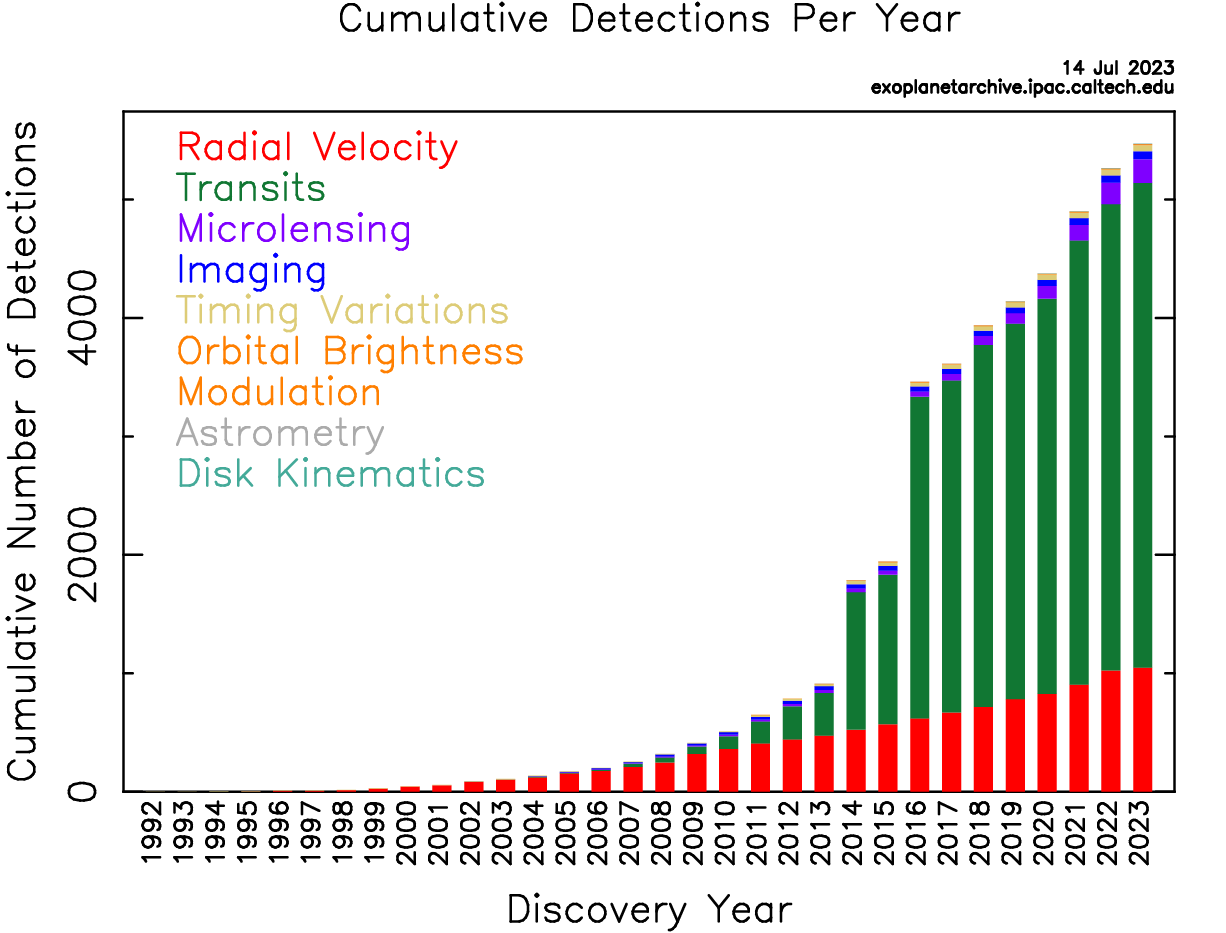
\includegraphics[width=1\linewidth]{image/dischist_cumulative.png}
    \captionsetup{font=small} 
    \caption{Discovery of Exoplanets: The first exoplanet around a Solar-type star was discovered by using the radial velocity technique in 1995. This technique is the most important approach to detect exoplanets from 1995 to 2010. After that, a more efficient technique was developed, named Transits, which accelerated the discovery of exoplanets. Until now, there are more than 5,000 exoplanets have been detected and confirmed. Other techniques contributed to the detection of exoplanets as well.}
    \label{fig:dischist_cumulative}
\end{figure}
\vspace{\baselineskip}
The diversity and complexity of exoplanets have also become apparent through comparisons with planets in our solar system. By referring to the NASA exoplanet archive, three key plots can help illustrate this diversity.

\begin{figure}[H]
    \centering
    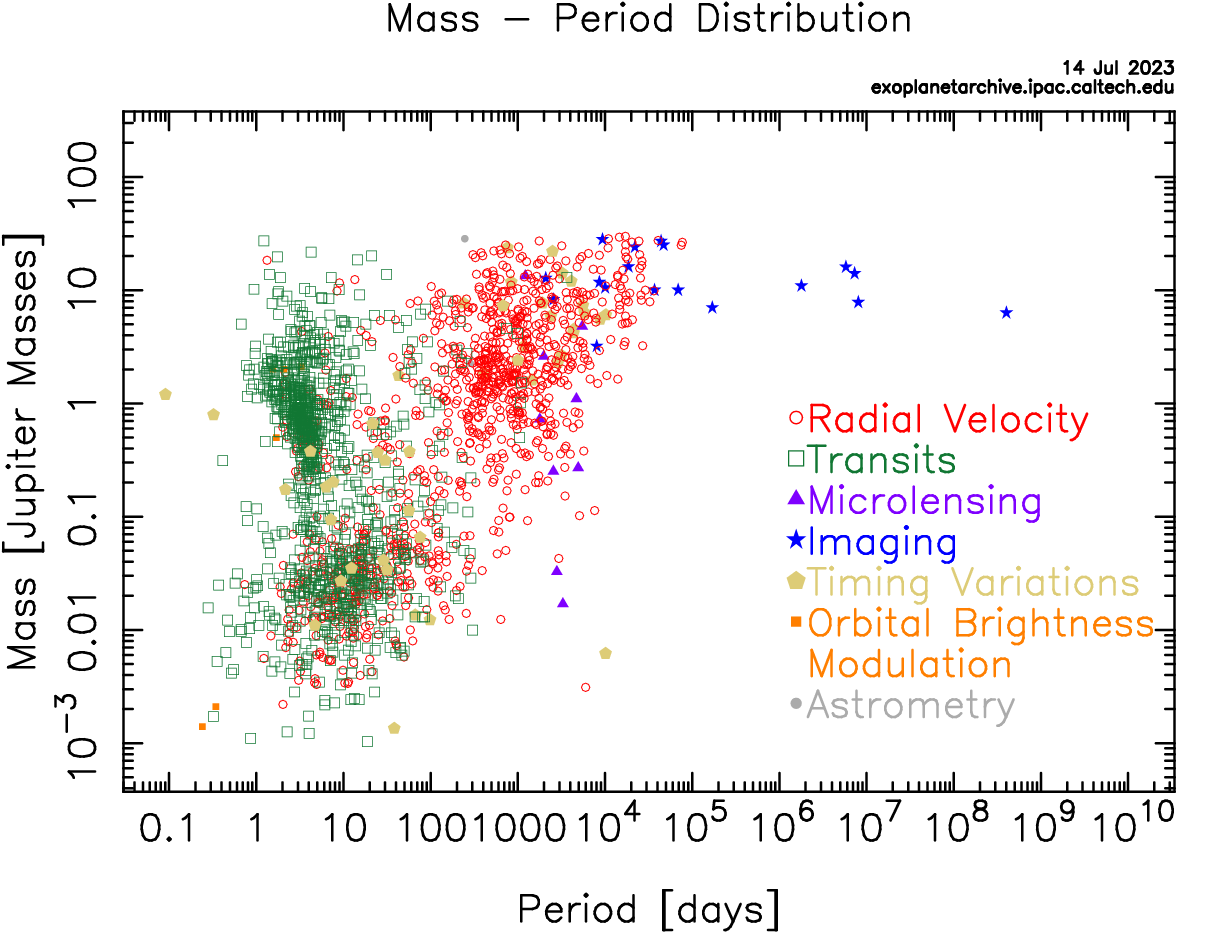
\includegraphics[width=1\linewidth]{image/mass_period.png}
    \captionsetup{font=small} 
    \caption{The distribution of orbital periods versus planetary mass}
    \label{fig:mass_period}
\end{figure}

The Figure~\ref{fig:mass_period} shows the distribution of orbital periods versus planetary mass. It reveals a wide range of planetary groups, from gas giants to super-Earths and even rocky planets. The distribution of orbital periods also varies, with some exoplanets having short periods comparable to days or weeks, while others have long orbital periods spanning several years. The discovery of short-period, massive exoplanets challenges previous notions of planetary formation in the solar system. Hot Jupiter's close orbits raise questions about migration and planetary dynamics. This groundbreaking research, recognized by the 2019 Nobel Prize in Physics, expands our understanding of exoplanetary systems.

\begin{figure}[H]
    \centering
    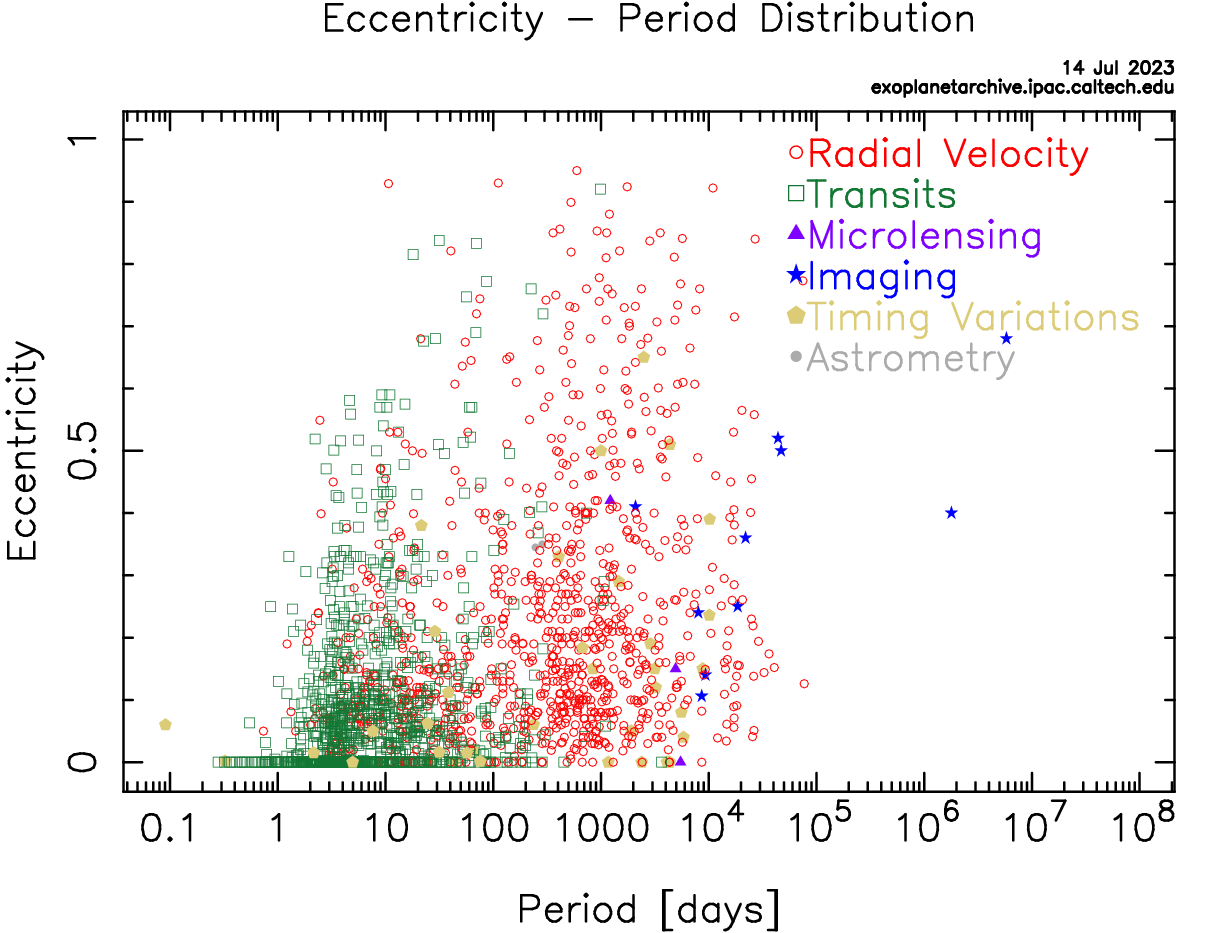
\includegraphics[width=1\linewidth]{image/ecc_period.png}
    \captionsetup{font=small} 
    \caption{The relationship between the orbital period and eccentricity}
    \label{fig:ecc_period}
\end{figure}

The Figure~\ref{fig:ecc_period} displays the relationship between the orbital period and eccentricity. It demonstrates that exoplanets exhibit a broad range of eccentricities, from nearly circular orbits (low eccentricity) to highly elliptical orbits (high eccentricity). This diversity in eccentricity suggests a variety of formation and dynamical processes in exoplanetary systems.

\begin{figure}[H]
    \centering
    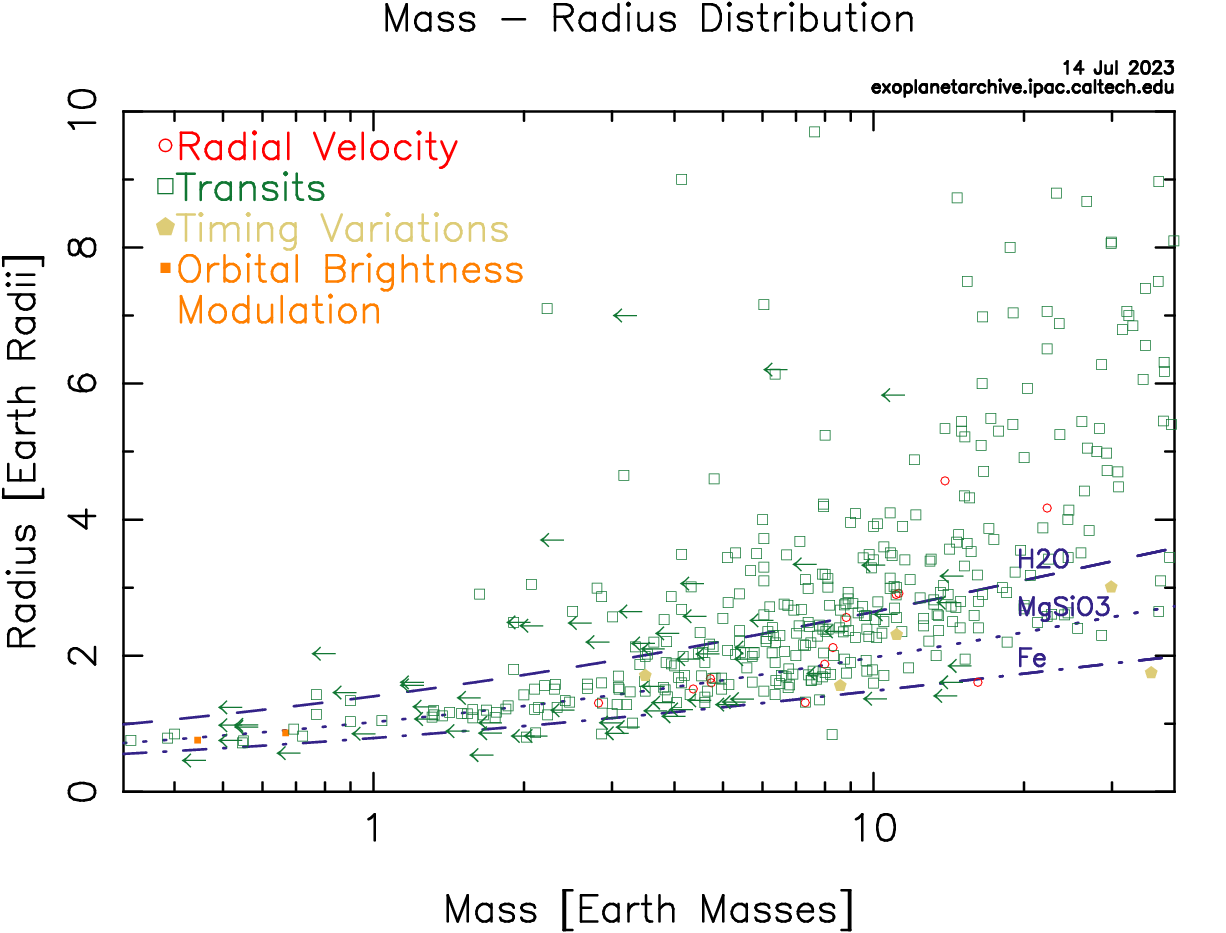
\includegraphics[width=1\linewidth]{image/mass_radius.png}
  \captionsetup{font=small} 
    \caption{Planetary mass versus radius reveals intriguing}
    \label{fig:mass_radius}
\end{figure}

Lastly, the Figure~\ref{fig:mass_radius} showcasing planetary mass versus radius reveals intriguing patterns. While there is a general trend of increasing planet size with higher groups, there are notable exceptions. Some exoplanets defy expectations by having unexpectedly low densities or inflated sizes, challenging our understanding of their internal structure and composition.

These plots highlight the incredible diversity and complexity of exoplanetary systems, revealing a rich tapestry of planetary characteristics that extend beyond our solar system. Continued observations and analyses will undoubtedly unveil further surprises and deepen our understanding of exoplanets, paving the way for exciting discoveries in the quest for extraterrestrial life and our place in the universe.

\subsection{Exoplanetary Atmosphere}

Exoplanetary atmospheres are extremely important in shaping a planet's features and habitability. Understanding how a planet's atmosphere affects its surface temperature requires measuring the emissivity, or reflectivity, of the atmosphere. A framework for calculating surface temperature, a key indicator for researching planetary habitability, is provided by the Stefan-Boltzmann formula. Additionally, a planet's emissivity may be used to deduce the chemical makeup of its atmosphere, revealing details about its atmospheric characteristics and the likelihood that it might harbor life.

There are various difficulties in measuring the emissivity of exoplanets. Since atmospheric impacts frequently cause tiny brightness variations, finding them requires a high level of accuracy. Our strategy relies on the Transiting Exoplanet Survey Satellite's (TESS) high-precision photometry to get around these difficulties. TESS continually monitors the brightness of many stars, making it possible to spot even tiny changes brought on by exoplanetary transits. Scientists can measure the emissivity of exoplanets and learn important details about their atmospheric makeup and potential habitability by carefully researching these fluctuations.

TESS's high-precision photometry and its ability to monitor a large number of stars make it an invaluable resource for studying exoplanetary atmospheres. The mission's extensive observations have provided significant contributions to our understanding of exoplanets and have helped identify targets for more detailed follow-up studies using advanced telescopes and instruments.

Further developments in observational technologies and data analysis approaches will improve our capability to assess exoplanetary atmospheres as exoplanet science advances. These observations will further our knowledge of the prerequisites for habitability and the possibility of life outside of our Solar System by providing insights into the wide variety of atmospheres present in exoplanetary worlds.

\section{Theories}

\subsection{Planetary Transit}

Planetary transit is an important method for detecting and studying exoplanets. The probability of a transit occurring depends on the size of the planet, the inclination of its orbit, and the size of the host star. On the light curve, the theoretical transit profile can be modeled using a simple model and a more complex model that incorporates the limb-darkening effect. The simple model assumes the planet fully blocks the star without considering other factors. The transit profile can be modeled as an eclipse of a spherical star by an opaque, dark sphere. In what follows, d is the center-to-center distance between the star and the planet, $r_{p}$ is the radius of the planet, $r_{*}$ is the stellar radius, $z = d/r_{*}$ is the normalized separation of the centers, and $p = r_{p}/r_{*}$ is the size ratio. The flux relative to the unobscured flux is $F$. For a uniform source, the ratio of obscured to unobscured flux is $F^{e}(p,z) = 1- \lambda^{e}(p,z)$, where

\begin{equation}
\label{uniformoccult}
\lambda^e(p,z) = 
\left\{\begin{array}{ll}
0  &  1+p < z \\\frac{1}{\pi} \left[p^2 \kappa_0+\kappa_1-\sqrt\frac{4z^2-(1+z^2-p^2)^2} {4}\right] &  |1-p| < z \le 1+p \\
 p^2 & z \le 1-p\\
1  &  z \le p-1,\\
\end{array}\right.
\end{equation}

and $\kappa_{1} = cos^{-1}[(1-p^2+z^2)/2z]$, $\kappa_{0} = cos^{-1}[(p^2+z^2-1)/2pz]$. 
\vspace{\baselineskip}

\begin{figure}[H]
    \centering
    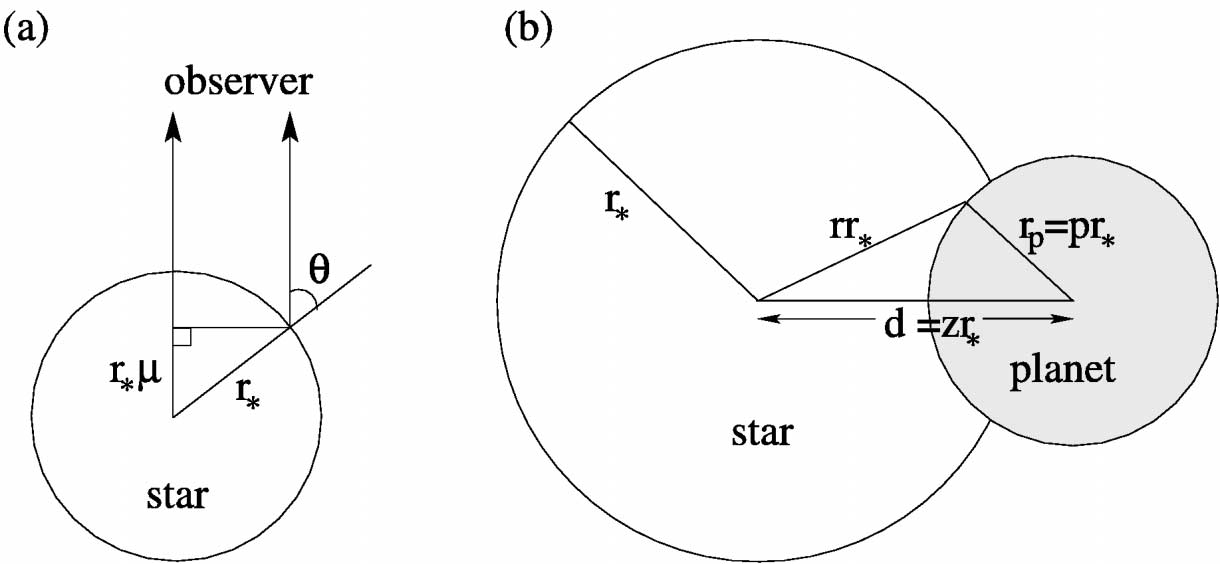
\includegraphics[width=0.9\linewidth]{image/sample_eclipse_model.png}
    \captionsetup{font=small} 
    \caption{Geometry modeling of transit: (a) The star is seen edge-on, with the observer off the top of the page. The star has radius $r_*$, and $\theta$ is defined as the angle between the observer and the normal to the stellar surface, while $\mu = cos\theta$. (b) Transit geometry from the perspective of the observer.}
    \label{fig:sem_alc}
\end{figure}
\vspace{\baselineskip}
This model neglects the limb-darkening effect and only considers the geometrical shape of the planet and star.

However, in actual observations, the limb-darkening effect plays a significant role in the light curve. To model the transit profile more accurately, complex theoretical models consider the geometrical shape of the planet and star, atmospheric transmissivity, and the limb-darkening effect. By incorporating limb darkening coefficients, we can plot the theoretical transit profile considering the limb darkening effect. Such plots demonstrate the variations in flux during the transit event and provide valuable information about the planet's characteristics. The accompanying presents an example plot that includes the theoretical transit profile. The plot shows the changes in flux during the transit event and the influence of limb darkening on the brightness distribution of the star. This analysis aids in understanding the light curve and serves as a benchmark for comparing observed data with theoretical models. By combining the simple model with the more complex model incorporating limb darkening, we can better understand the phenomenon of planetary transits and extract essential information about the planet. This is crucial for revealing the physical properties and atmospheric composition of exoplanets, advancing our understanding of their formation and evolution processes. In our project, we are researching the basic planetary transit, limb-darkening is not the focus and is considered in our modeling code.

\subsection{Secondary Eclipse and Day-night Modulation}

In the light curves of exoplanets, two atmospheric-related phenomena with comparable amplitudes are secondary eclipse and day-night modulation. A planet's total eclipse by its host star while it is in its orbit is referred to as a secondary eclipse. On the other hand, day-night modulation depicts the fluctuations in light brought on by the planet's rotation.

Using light curve analysis, theoretical profiles for secondary eclipses and day-night modulation may be created. The size of the planet, orbital inclination, and size of the host star may all be used to predict the depth and length of secondary eclipse occurrences. Additionally, these models can account for atmospheric transmissivity as well as potential impacts from atmospheric absorption and scattering.

It is possible to find theoretical profiles for secondary eclipses by consulting material in the Exoplanet Handbook. These profiles demonstrate how flux varies over time and identify the planet that is being shadowed by its star. It is possible to conclude the planet's atmospheric characteristics and composition by contrasting observational data with theoretical models.

\begin{figure}[H]
    \centering
    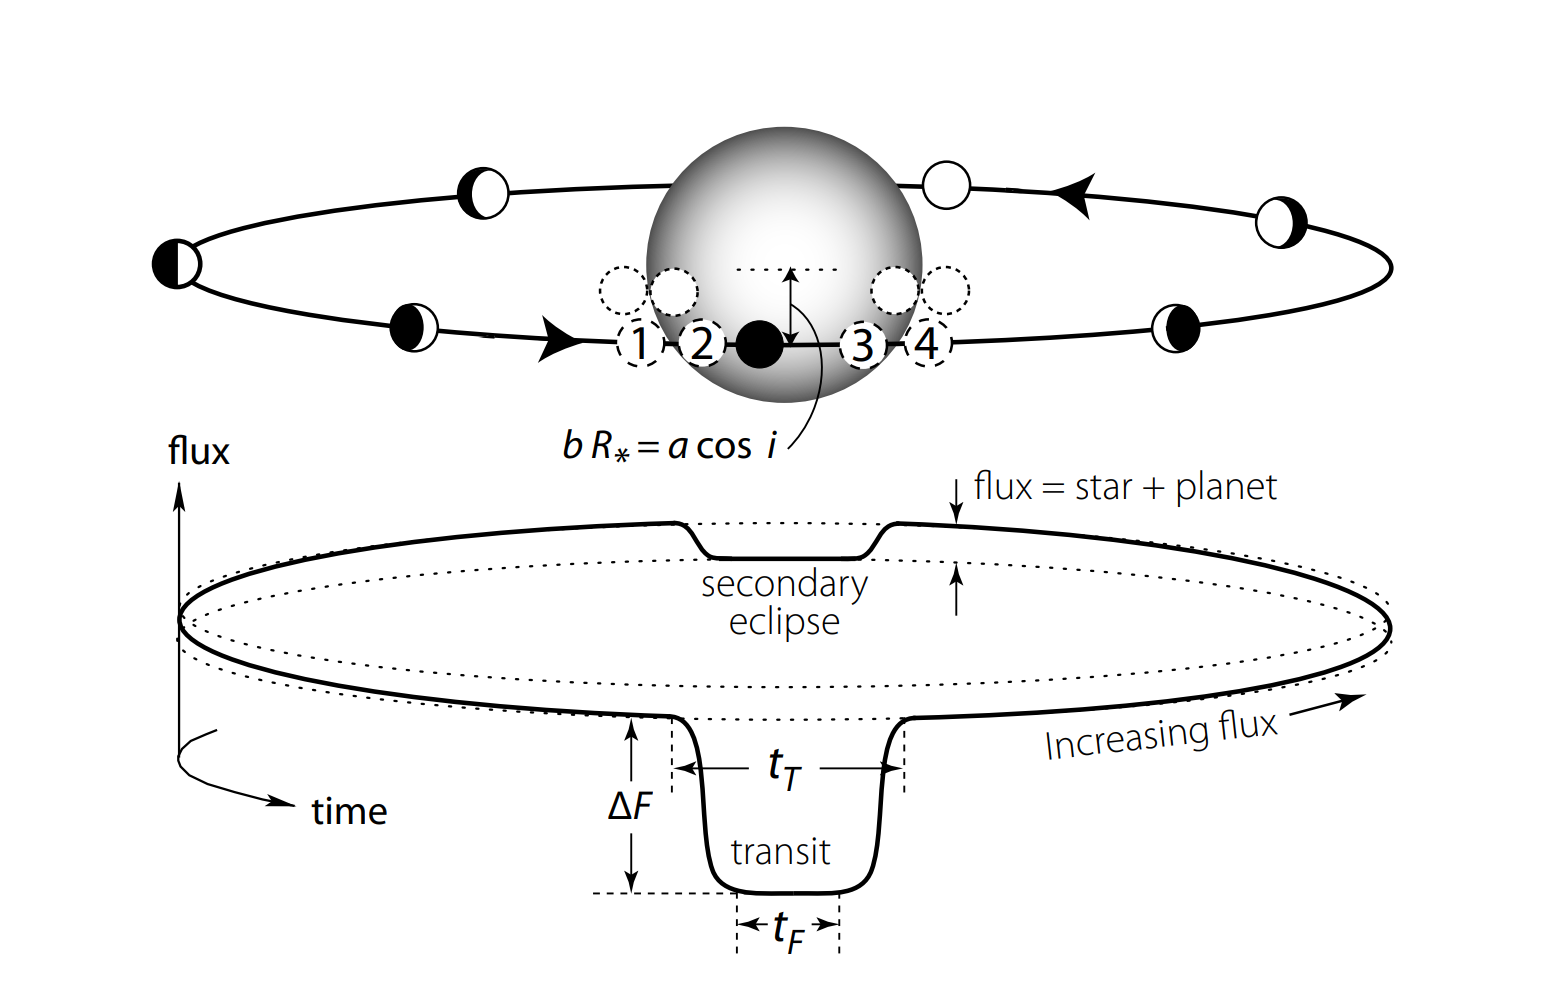
\includegraphics[width=1\linewidth]{image/transit_sample_model.jpg}
    \captionsetup{font=small} 
    \caption{Schematic of a transit. During the transit, the planet blocks a fraction of the starlight. After the transit, the planet’s brighter day-side progressively comes into view, and the total flux rises. It drops again during the secondary eclipse as the planet passes behind the star. Dashed circles show first to fourth contact points; those for smaller impact parameters (dotted) are more closely separated in time, and the ingress/egress slopes are correspondingly steeper. The total transit duration $t_{T}$ is between the first and fourth contact, while $t_{F}$ is timed between the second and third contact.}
    \label{fig:transit_sm}
\end{figure}

Similar to this, theoretical methods may be used to model day-night modulation. The observed day-night patterns are caused by brightness changes caused by the planet's rotation in various locations. Predictions for the magnitude and timing of the day-night modulation may be made by modeling the planet's rotating speed and atmospheric optical characteristics.

Understanding the effects of secondary eclipses and day-night modulation on the light curves is made more accessible by the use of theoretical models. These events offer essential insights into the properties, dynamics, and energy distribution of exoplanet atmospheres. We can learn more about the climate, air circulation, and probable seasonal changes of the earth by analyzing these patterns. This helps to reveal the characteristics of the planet's surface and atmosphere and offers crucial hints for examining planetary habitability.

\subsection{Ellipsoidal Variations and Doppler Beaming}

Ellipsoidal variations and Doppler beaming are two fascinating phenomena observed in the light curves of some binary star systems containing a close-in massive exoplanet or brown dwarf.

Ellipsoidal variations occur due to the tidal forces between the companion object (exoplanet or brown dwarf) and the host star. These forces cause the lead to become distorted into an elongated, ellipsoidal shape as the companion orbits around it. As a result, the observed brightness of the star varies periodically as the long star rotates, creating a characteristic sinusoidal pattern in the light curve.

Doppler beam, also known as Doppler boosting or Doppler effect, is a relativistic effect caused by the motion of the star due to the gravitational pull of the companion object. As the star moves toward us during its orbital motion, its light is slightly blue-shifted, making it appear slightly brighter. Conversely, when the star moves away from us, its light is red-shifted, making it appear slightly fainter. This periodic change in the star's brightness creates a distinctive modulated pattern in the light curve.

Both ellipsoidal variations and Doppler beaming are typically observed in binary systems where the companion object is massive and orbits closely around the host star. These effects can be measured and used to determine various parameters of the binary system, such as the mass and size of the companion object, the inclination of the orbit, and even the system's orientation concerning Earth.

\begin{figure}[H]
    \centering
    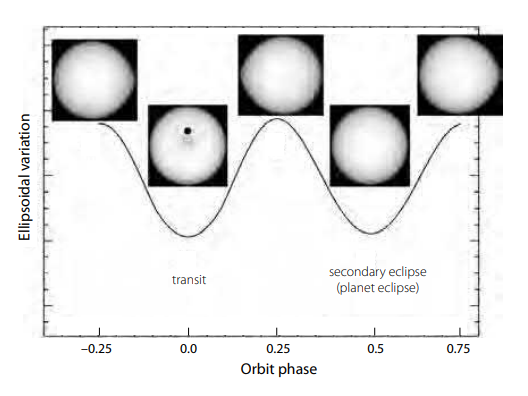
\includegraphics[width=0.9\linewidth]{image/orbit_ph.jpg}
    \captionsetup{font=small} 
    \caption{Schematic of ellipsoidal variations (arbitrary units) versus orbit phase. Phase 0 shows the planet during transit (transit signature not included), phases –0.25 and 0.25 at quadrature, and phase 0.75 at the secondary eclipse. From Jackson et al. (2012b, Figure 2), by permission of IOP Publishing/AAS.}
    \label{fig:ob_ph}
\end{figure}

\begin{equation}
    F = 1 - A_{ellip}\cos(2\phi) + A_{Dopp}\sin(\phi) + A_{dn}\cos(\phi)
\end{equation}

Studying these phenomena provides valuable information about the dynamics and characteristics of binary star systems containing massive companions. Moreover, the detection and analysis of ellipsoidal variations and Doppler beaming contribute to a better understanding of the properties and behavior of exoplanets and brown dwarfs in close orbits around their host stars.

\section{Data Collection}

\subsection{Transiting Exoplanet Survey Satellite}

The Transiting Exoplanet Survey Satellite (TESS) is a space telescope designed to search for exoplanets using the transit method. TESS employs a unique "staring mode" observation, continuously monitoring a fixed field of view covering approximately 24 and 96 degrees in the sky. The sky is divided into 28 "sectors" regions, each observed for about 27 days before shifting to the next sector, resulting in full-sky coverage. TESS ensures continuity by following each sector for multiple orbits, capturing potential transits or stellar variability over an extended period. With a high photometric cadence of every 2 minutes, TESS can detect short-duration transit events and monitor stellar variability.

\begin{figure}[H]
    \centering
    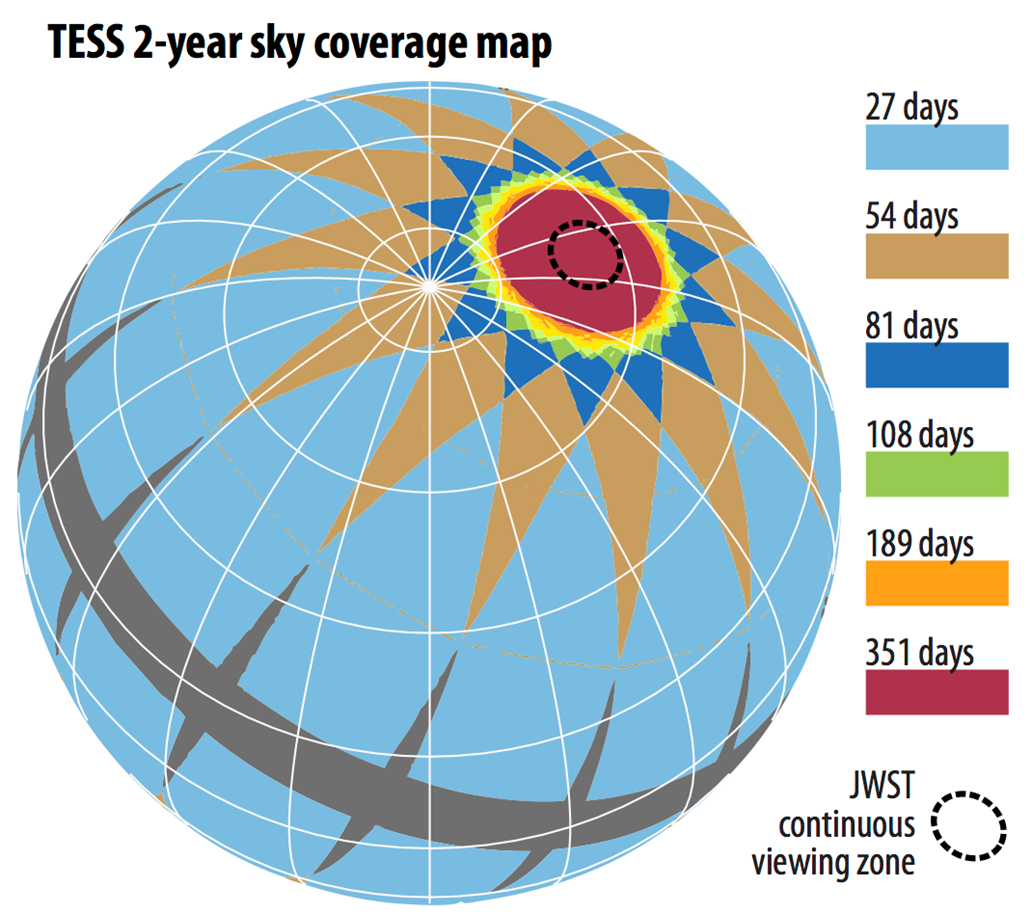
\includegraphics[width=0.6\linewidth]{image/sky_coverage.png}
    \captionsetup{font=small} 
    \caption{TESS will tile the sky with 26 segments, observing the southern hemisphere in the first year of mission operation and the northern hemisphere in the second year. TESS has a unique, 13.7 day,  highly elliptical cislunar orbit about Earth. With a 27.4-day observing period per segment, the satellite is most sensitive to exoplanets with periods of less than 13 days (so that at least two transits are used for discovery). The circular regions where segments overlap at the ecliptic poles have an observing period of just over 100 days, enabling longer-period planets to be discovered. These regions are known as continuous viewing zones (CVZs).}
    \label{fig:sky_cov}
\end{figure}

One of TESS's remarkable strengths is its ultra-high photometric precision, achieving an accuracy of up to one part in 100,000 for the brightest stars. This precision enables the detection of even small changes in brightness, essential for discovering Earth-sized planets around nearby stars. TESS's capabilities have led to the discovery of thousands of exoplanet candidates, contributing significantly to our understanding of exoplanetary systems and expanding the search for potentially habitable worlds beyond our solar system. TESS's continuous monitoring and high photometric cadence have significantly increased the volume and precision of exoplanetary data. This unprecedented wealth of information has revolutionized our understanding of exoplanets and their characteristics.

\subsection{TESS Objects of Interest Catalog}

The TESS Objects of Interest Catalog (TOI) plays a crucial role in our research as we leverage the valuable data the Transiting Exoplanet Survey Satellite (TESS) mission provides. With its comprehensive collection of astronomical objects, the TOI catalog offers 461 planets of essential parameters, mainly focusing on exoplanet candidates detected through the transit method. This data includes identification numbers, sky coordinates, host star brightness, and orbital periods of candidate exoplanets.

\begin{figure}[H]
    \centering
    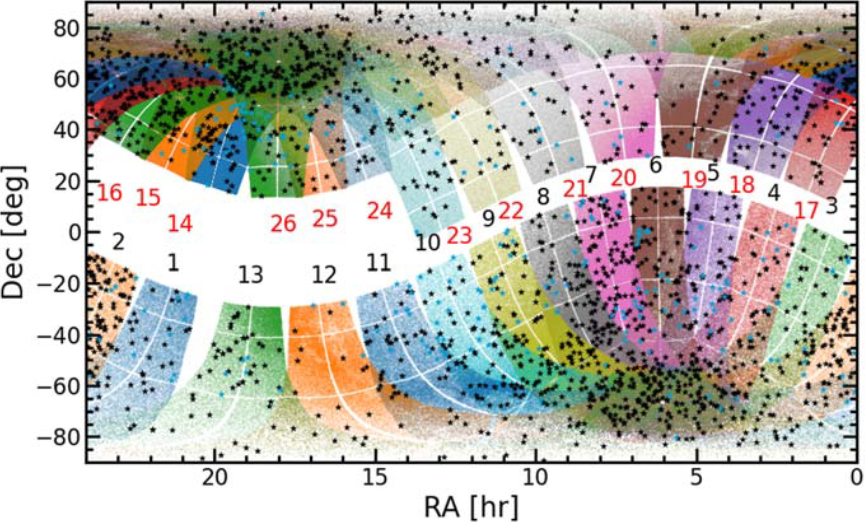
\includegraphics[width=1\linewidth]{image/catalog_dis.png}
    \captionsetup{font=small} 
    \caption{Sky positions of the TESS Prime Mission TOIs. The R.A. is on the horizontal axis, and decl. is on the vertical axis. The black points are TOIs. The blue points are previously known planets (NASA Exoplanet Archive, accessed 2020 August 14). The points within the multicolored swaths are stars (Tmag < 13.5) observed in the TESS Prime Mission. Fewer TOIs appeared in sectors 11 and 12 because the FOV was crowded, and this limited the number of viable TCEs for vetting.}
    \label{fig:dis_cata}
\end{figure}

Beyond exoplanet candidates, the TOI catalog encompasses information on various transient and variable objects, such as stellar binaries and pulsating stars, exhibiting periodic brightness variations. Continuously updated with new TESS observations, the TOI catalog constantly expands, offering us a growing array of objects of interest.

As researchers, we rely on the TOI catalog to identify potential targets for further observation, follow-up studies, and detailed characterization of exoplanet candidates and intriguing celestial phenomena. This invaluable resource enhances our understanding of exoplanets, stellar systems, and the diverse wonders of the universe. By harnessing the data from the TOI catalog, we contribute to advancing knowledge in exoplanet research and stellar astrophysics.

\subsection{Data file}

The TESS light curve files contain the time-series photometric measurements for analyzing exoplanet transits, eclipses, and stellar variability. As documented in the TESS Archive Manual (EXP-TESS-ARC-ICD-038), these Flexible Image Transport System (FITS) files have a structure comprising three Header Data Units (HDUs) (Extra material Table \hyperref[fig:table13]1\textcolor{blue}{3}):

\begin{figure}[H]
    \centering
    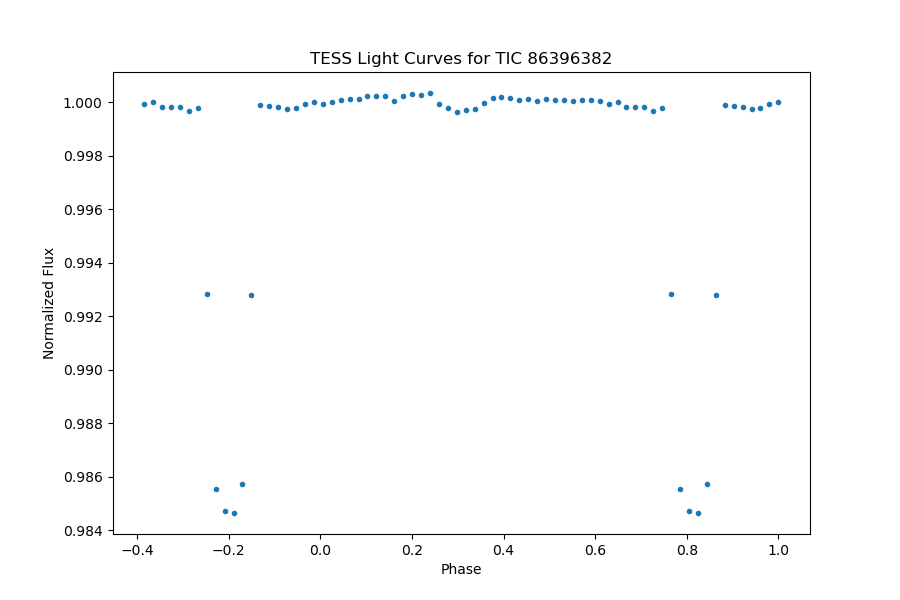
\includegraphics[width=1\linewidth]{image/86396382_folded.png}
    \captionsetup{font=small} 
    \caption{A sample of data file. This object TIC 86396382 or WASP12B has been well researched and has a typical light curve of planet transit secondary eclipse and day-night modulation.}
    \label{fig:wasp12b}
\end{figure}

\begin{itemize}

    \item Primary HDU: Includes metadata such as the celestial coordinates of the target, sector/camera designations, and aggregate data quality flags.

    \item 1st Extension HDU: Contains binary FITS tables storing the time-series photometry, with columns for Barycentric Julian Dates (BJDs) (TIME), Simple Aperture Photometry (SAP) flux values (SAP FLUX), SAP flux uncertainties (SAP FLUX ERR), and other parameters.

    \item 2nd Extension HDU: An image extension with the pixel data used for photometric extraction.
    
\end{itemize}

For our analysis, the key columns are:

\begin{itemize}

    \item TIME: Barycentric Julian Dates in TESS Barycentric Julian Date (TBJD) format, providing time stamps for each flux measurement.

    \item SAP FLUX: The target's brightness is measured within the optimal aperture at each time stamp, in units of electrons per second.

    \item SAP FLUX ERR: The uncertainties in the SAP FLUX values propagated through the entire photometric pipeline.

    \item QUALITY: Integer flags indicating compromised or anomalous data points requiring cautious treatment or exclusion.
    
\end{itemize}

By extracting these columns using astropy FITS utilities, we can construct light curves and assess data quality based on the QUALITY flags. Careful screening of measurements via these flags is imperative before modeling and interpretation.

\section{Analysis of Light Curve}

\subsection{Planetary Transit fitting}

Fitting the photometric light curves of planetary transit events is crucial for deriving the physical parameters of the planet-star systems. Our methodology encompasses.

\begin{itemize}

    \item Constructing physical models of the transit events. Standard analytic models include those by Mandel and Agol (2002) and Torres et al. (2008) incorporating nonlinear limb darkening. The models contain parameters like transit mid-point T0, orbital period P, planet-star geometric configurations, etc.

    \item Extracting the time (TIME) and flux (SAP FLUX) columns from the TE
    SS light curve files using astropy FITS utilities.

    \item Utilizing nonlinear least squares fitting routines in Scipy to fit the observed light curves and derive optimal model parameters.

    \item Assessing consistency of fitted parameters with literature values. For WASP-12b, the held orbital period of 1.09142 days agrees well with the Gaia DR2 value of 1.091414 days.

    \item Evaluating goodness-of-fit via residuals inspection and reduced chi-squared. Good fits yield residual distributions close to Gaussian and reduced chi-squared values near unity. 
    \item Probing parameter inter-dependencies, e.g., through MCMC posterior distributions.
    
\end{itemize}

In practice, suitable models are chosen flexibly for each planetary system. Additionally, the treatment of systematic noise is critical in the fitting process. Overall, delicate light curve fitting enables the determination of system parameters, model evaluation, and foundations for further analysis.

\subsection{Fine processing of TESS light curve}

Fine processing refers to the additional corrections and filtering applied to the raw photometry after initial light curve extraction, to mitigate instrumental systematics and abnormal values, yielding light curves amenable to in-depth scientific analysis.

\begin{figure}[H]
    \centering
    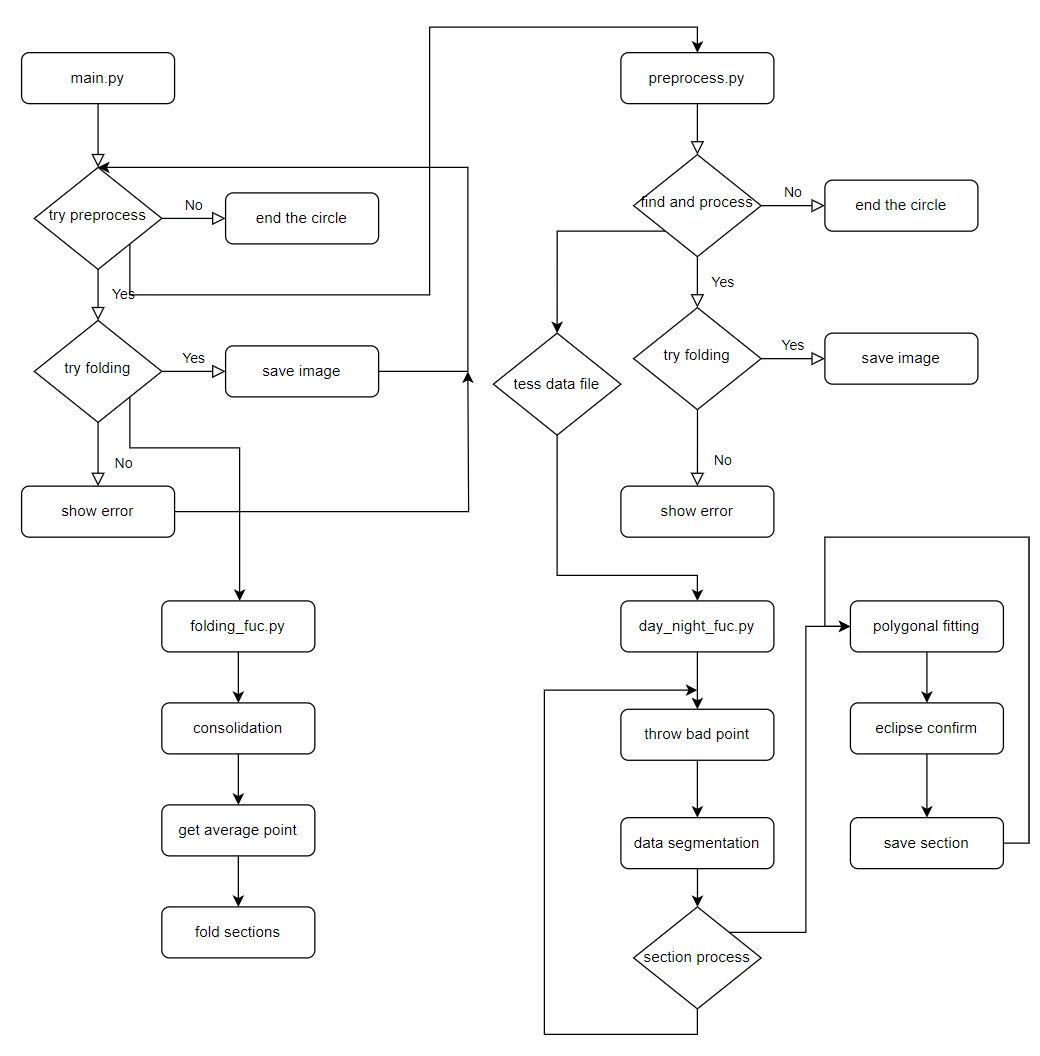
\includegraphics[width=0.8\linewidth]{image/code_process.jpg}
    \captionsetup{font=small} 
    \caption{This graph shows how specific the Python code is running including every major step, function, and file. A logical and stable Python program was made during our research. We have spent much time mixing the bug of the automatic process of folding the Tess light curve. Eventually, it made us able to analyze 461 objects and get 17 objects that have fantastic secondary eclipse light curves. Our codes are now open source on GitHub (View TabNahida's Project about TESS) which means that every researcher can use them easily and do less redoing process.}
    \label{fig:code_p}
\end{figure}

\subsubsection{Key steps in fine processing}

\begin{itemize}

    \item Detrending: Removing long-term trends in the light curves to flatten them to a standardized baseline level. Polynomial fitting is commonly implemented for detrending.

    \item Gap filling: Interpolating across gaps in the data due to orbital interrupts, instrument anomalies, etc. to provide complete phase coverage.

    \item Outlier rejection: Scrutinizing quality flags (QUALITY) to excise photometric measurements tagged as problematic.

    \item Filtering: Applying smoothing filters (e.g. Savitzky-Golay filter) to attenuate high-frequency noise in the time series data.

    \item Normalization: Standardizing the light curves to enable comparison of transit depths across different targets.
    
\end{itemize}

\subsubsection{Batch processing}

\begin{itemize}

    \item Modular functions encapsulating the exemplary processing steps can be constructed and assembled into a pipeline for automated bulk processing of numerous light curves.

    \item Leveraging Python's multiprocessing and parallel computing tools can significantly accelerate the processing by parallelizing tasks.
    
\end{itemize}

\subsubsection{Evaluation} 

\begin{itemize}

    \item Cross-validating parameters against literature for correctness.

    \item Quantifying noise reduction via RMS before and after.

    \item Checking if variability signals are enhanced in clarity.
    
\end{itemize}

Please review this outline and suggest any modifications. I would be happy to refine the details of this section further. Thank you!

\subsection{Detection of orbital phase variations}

Fold the long baseline photometric time series into a complete orbital phase cycle. This can be achieved by computing the phase for each timestamp based on the transit ephemeris. Secondary eclipses and day-night flux modulations induced by the planetary atmosphere are observable in the phase-folded light curve. Secondary eclipses manifest as a depression around phase 0.5 as the planet passes behind the host star. Day-night variations display a double-peaked sinusoidal pattern over the orbital phase due to the planet's rotation. Ellipsoidal variations and Doppler beaming arising from the host star's motion also induce quasi-sinusoidal signals in the light curve that need to be disentangled from the planetary movements. Ellipsoidal variations are caused by the tidal distortion of the star by the planet. Doppler beaming is a relativistic boosting effect due to the star's orbital motion.  Construct models comprising the above components and incrementally adjust the parameters until an optimal fit to the observed data is attained. Typical free parameters include the secondary eclipse depth, day-night modulation amplitude, ellipsoidal variation semi-amplitude, etc. Evaluate the relative quality of fit for different models using statistical criteria like the Bayesian Information Criterion to determine the best-matching model. Assess the significance of each effect. Derive the parameter values and uncertainties from the optimal model fit. Compare the retrieved deals against literature reports to validate the results. Uncertainties can be estimated using techniques like Markov Chain Monte Carlo. Perform model-checking procedures to ensure the residuals from the fit do not display any systematic structure. Assessment of the residuals can help identify additional effects that may need to be incorporated into the model. Carry out posterior predictive checks by generating simulated data points from the fitted model and comparing summary statistics between the simulated and observed data. 

\section{Sample Analysis}

\subsection{Sample selection}

Out of 461 TESS objects, we identified an optimal sample of 17 exoplanets exhibiting substantial secondary eclipses and day-night flux variability indicative of atmospheric dynamics. Our rigorous selection criteria were:

\begin{itemize}
    \item Orbital period $<$ 5 days - Shorter periods increase the likelihood of reflected light signatures.
    
    \item Transit depth $>$ 5000 ppm - Larger planet radii result in more pronounced atmospheric signals.

    \item Stellar magnitude $<$ 12 - Brighter host stars provide higher photometric precision.
    
\end{itemize}

We acquired the TESS light curve files for 461 candidate systems meeting the above criteria. Through batch preprocessing, we removed invalid data points, normalized the fluxes, and generated consistent high-quality photometric time series essential for our analysis.

To maximize the observational baseline, we stitched and phase-folded the multi-sector light curves using a finely tuned approach determined after extensive experimentation.

We then visually inspected the phase-folded curves to identify 24 exoplanets displaying significant secondary eclipse features, characterized by a depression in flux at phase 0.5 when the planet passes behind the host star.

Finally, we carried out rigorous model fitting of the phase-folded light curves to disentangle the day-night flux variability. Our final sample comprises 17 exoplanets exhibiting substantial secondary eclipses and coherent day-night photometric modulations attributable to longitudinal thermal gradients in their atmospheres.

In summary, we applied a rigorous, multi-step target selection process to systematically identify the optimal exoplanets from the TESS database for characterizing atmosphere dynamics through phase curve analysis.

\subsection{Results}

From our optimally selected sample of exoplanets, we present a detailed analysis of representative systems exhibiting different varieties of phase curve signals. These include clear secondary eclipses similar to WASP-12b and pronounced day-night flux modulations as observed in KELT-1b. Through refined light curve modeling, we accurately characterize these effects and properties revealed by the photometric variations over the orbital phase.

For each system, we phase-folded the TESS light curves on the transit period
Model secondary eclipses and day-night modulations
Account for stellar effects including ellipsoidal variations and Doppler beaming
Quantify the significance of detections
Derive implications from the fitted parameters
The remaining exoplanets in our sample did not exhibit significant phase curve signals, primarily due to stellar noise or insufficient photometric precision, though these null results also provide meaningful constraints.

Our analysis of select short-period giant exoplanets observed by TESS demonstrates the diverse conditions and physical processes revealed through phase curve modeling. From non-detections to prominent secondary eclipses and day-night variations, these systems showcase the insights enabled by high-precision, long-duration photometry. This work underscores the value of phase curve characterization for comprehensively probing exoplanetary properties through current and future missions.

In the graph below, they show different WASB 12 b-like with clearly secondary eclipse and day-night modulation TESS object and their analysis about what their light curve look like and why they are attractive.
\newpage

\subsubsection{Stars of TESS objects that have not only day-night modulation but also relativity of the exoplanet}

The planet TIC 16740101 has an orbital period of 1.481139064 days, showing significant transit with a depth of 0.00707179544\% and a transit duration of 3.982476435 hours. The secondary eclipse can be identified significantly in the full phase-folded light curve Figure \ref{fig:16740101_folded}. A close review of the light curve outside of transit Figure \ref{fig:16740101}, we fit the light curve with models of the secondary eclipse and day-night modulation.

\begin{figure}[H]\centering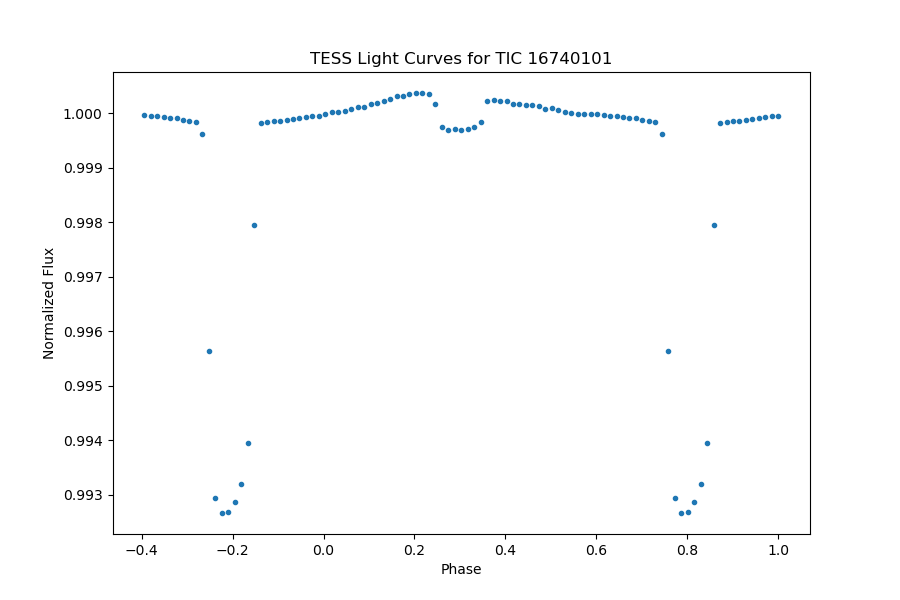
\includegraphics[width=0.7\linewidth]{image/16740101_folded.png}
\captionsetup{font=small} 
\caption{The full phase-folded light curve of TIC 16740101, planetary transit is very clear and the secondary eclipse can be identified significantly.}\label{fig:16740101_folded}\end{figure}\begin{figure}[H]\centering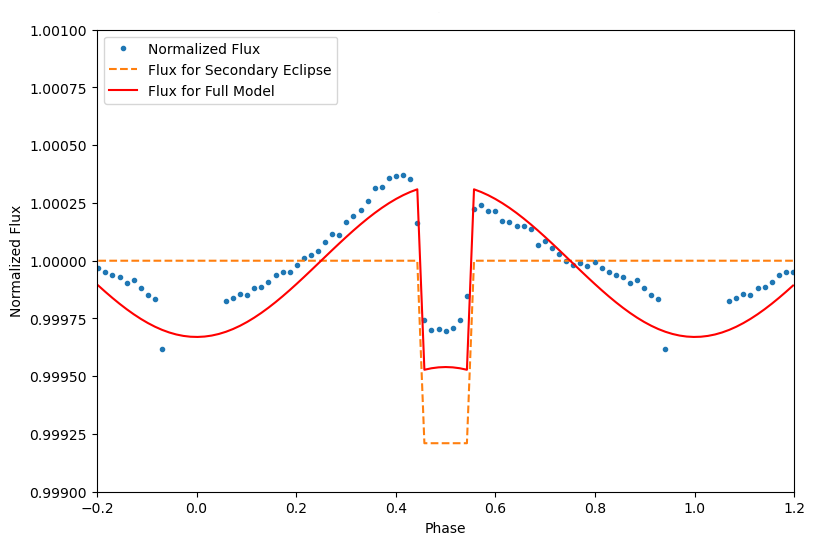
\includegraphics[width=0.65\linewidth]{image/16740101.png}
\captionsetup{font=small} 
\caption{A close review of the phase-folded light curve of TIC 16740101, the models of the secondary eclipse and day-night modulation are presented.}\label{fig:16740101}\end{figure}
\newpage
The planet TIC 86396382 has an orbital period of 1.0914167 days, showing significant transit with a depth of 0.01709\% and a transit duration of 2.774 hours. The secondary eclipse can be identified significantly in the full phase-folded light curve Figure \ref{fig:86396382_folded}. A close review of the light curve outside of transit Figure \ref{fig:86396382}, we fit the light curve with models of secondary eclipse and day-night modulation.\begin{figure}[H]\centering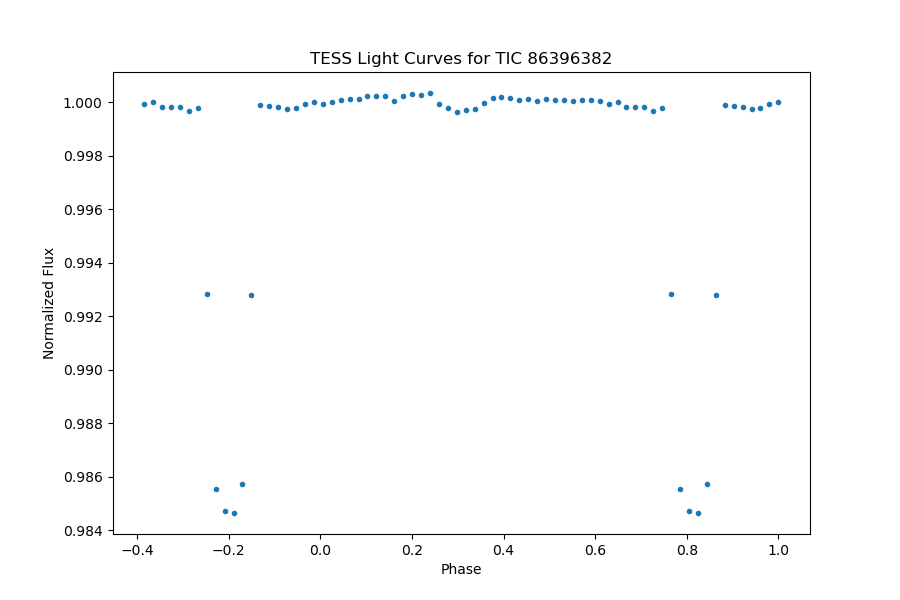
\includegraphics[width=0.7\linewidth]{image/86396382_folded.png}
\captionsetup{font=small} 
\caption{The full phase-folded light curve of TIC 86396382, planetary transit is very clear and the secondary eclipse can be identified significantly.}\label{fig:86396382_folded}\end{figure}\begin{figure}[H]\centering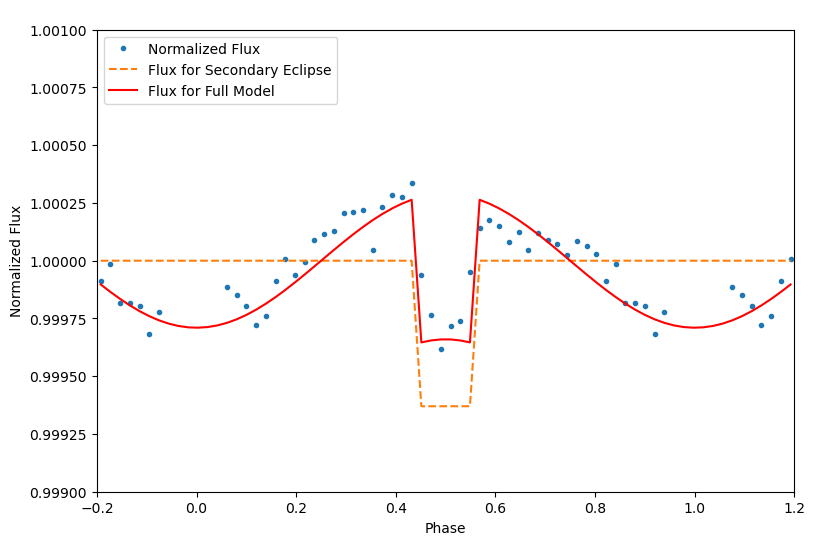
\includegraphics[width=0.65\linewidth]{image/86396382.png}
\captionsetup{font=small} 
\caption{A close review of the phase-folded light curve of TIC 86396382, the models of secondary eclipse and day-night modulation are presented.}\label{fig:86396382}\end{figure}
\newpage
The planet TIC 354619337 has an orbital period of 2.148787199 days, showing significant transit with a depth of 0.007058741068\% and a transit duration of 4.167148992 hours. The secondary eclipse can be identified significantly in the full phase-folded light curve Figure \ref{fig:354619337_folded}. A close review of the light curve outside of transit Figure \ref{fig:354619337}, we fit the light curve with models of secondary eclipse and day-night modulation.\begin{figure}[H]\centering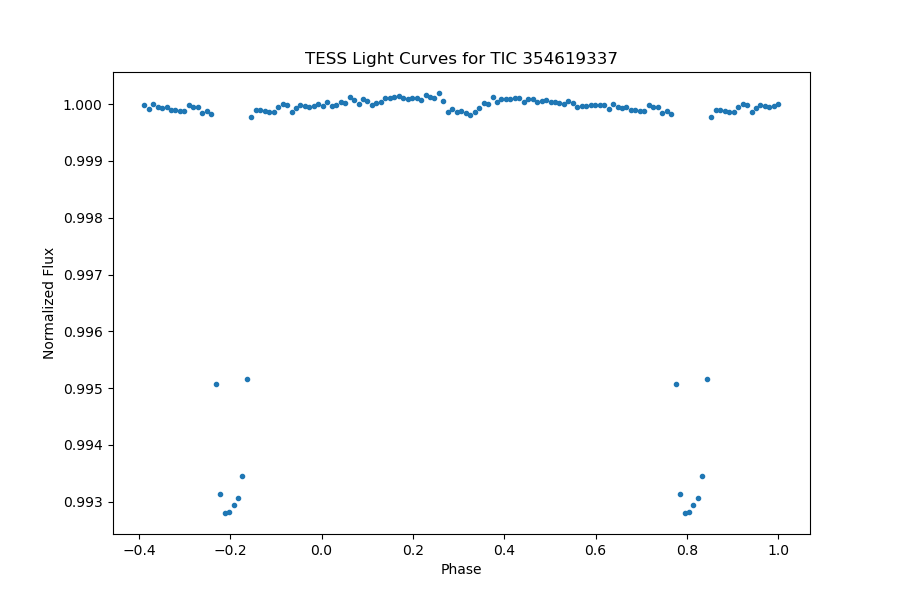
\includegraphics[width=0.7\linewidth]{image/354619337_folded.png}
\captionsetup{font=small} 
\caption{The full phase-folded light curve of TIC 354619337, planetary transit is very clear and the secondary eclipse can be identified significantly.}\label{fig:354619337_folded}\end{figure}\begin{figure}[H]\centering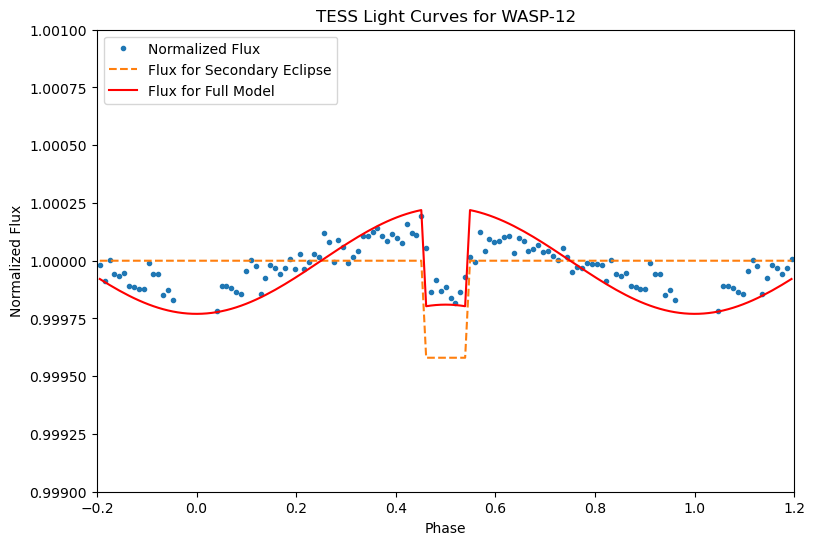
\includegraphics[width=0.65\linewidth]{image/354619337.png}\captionsetup{font=small} \caption{A close review of the phase-folded light curve of TIC 354619337, the models of secondary eclipse and day-night modulation are presented.}\label{fig:354619337}\end{figure}
\newpage
\subsubsection{TESS object with normal secondary eclipse}

The planet TIC 22529346 has an orbital period of 1.2749246 days, showing significant transit with a depth of 0.01885\% and a transit duration of 2.744 hours. The secondary eclipse can be identified significantly in the full phase-folded light curve Figure \ref{fig:22529346_folded}. A close review of the light curve outside of transit Figure \ref{fig:22529346}, we fit the light curve with models of the secondary eclipse and day-night modulation.\begin{figure}[H]\centering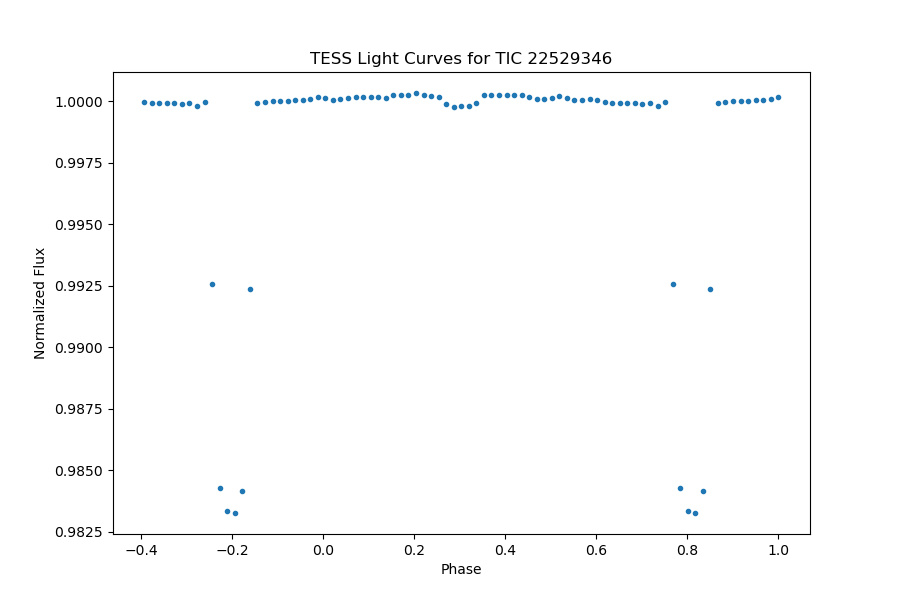
\includegraphics[width=0.7\linewidth]{image/22529346_folded.png}\captionsetup{font=small} \caption{The full phase-folded light curve of TIC 22529346, planetary transit is very clear and the secondary eclipse can be identified significantly.}\label{fig:22529346_folded}\end{figure}\begin{figure}[H]\centering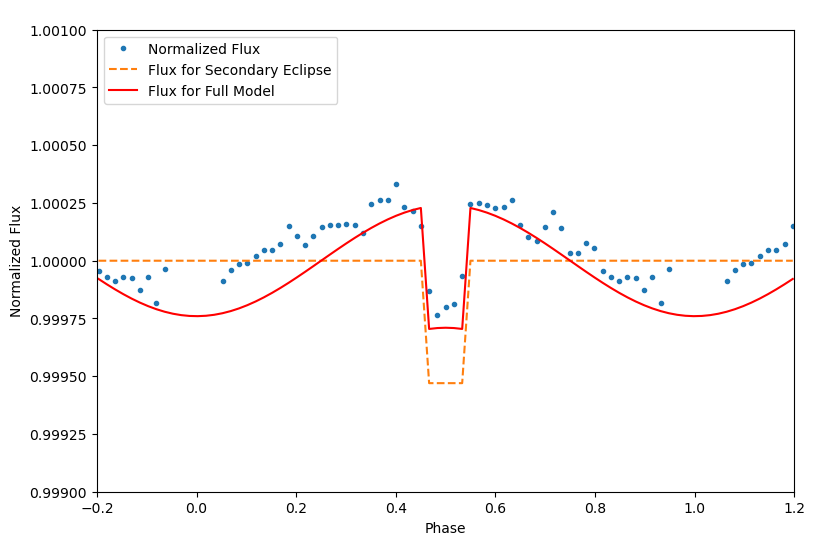
\includegraphics[width=0.65\linewidth]{image/22529346.png}\captionsetup{font=small} \caption{A close review of the phase-folded light curve of TIC 22529346, the models of the secondary eclipse and day-night modulation are presented.}\label{fig:22529346}\end{figure}
\newpage
The planet TIC 139528693 has an orbital period of 2.175172877 days, showing significant transit with a depth of 0.00778064352\% and a transit duration of 4.791880622 hours. The secondary eclipse can be identified significantly in the full phase-folded light curve Figure \ref{fig:139528693_folded}. A close review of the light curve outside of transit Figure \ref{fig:139528693}, we fit the light curve with models of secondary eclipse and day-night modulation.\begin{figure}[H]\centering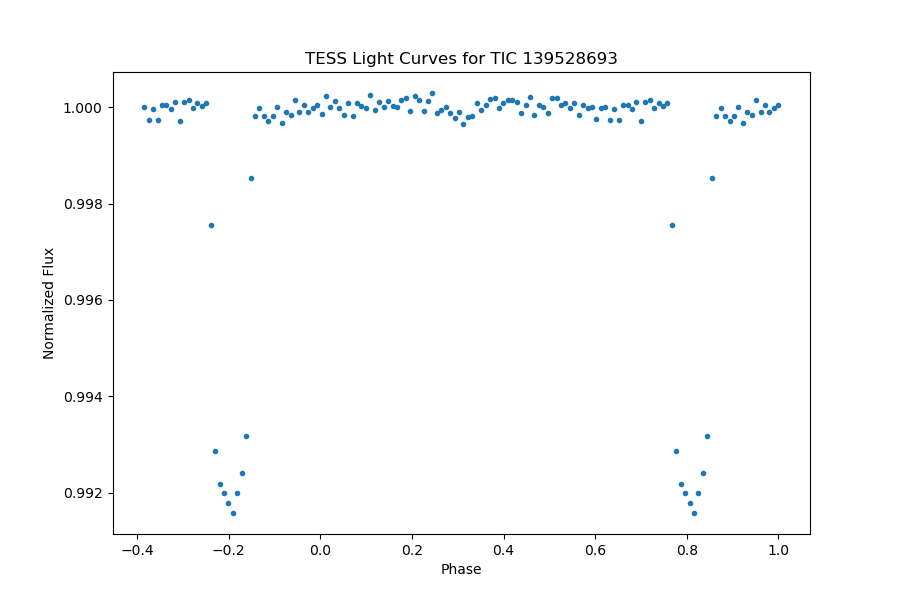
\includegraphics[width=0.7\linewidth]{image/139528693_folded.png}\captionsetup{font=small} \caption{The full phase-folded light curve of TIC 139528693, planetary transit is very clear and the secondary eclipse can be identified significantly.}\label{fig:139528693_folded}\end{figure}\begin{figure}[H]\centering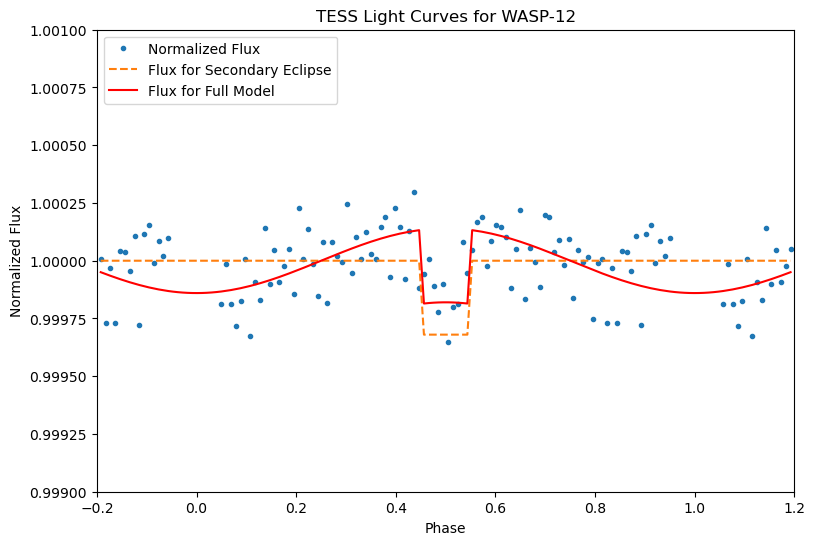
\includegraphics[width=0.65\linewidth]{image/139528693.png}\captionsetup{font=small} \caption{A close review of the phase-folded light curve of TIC 139528693, the models of secondary eclipse and day-night modulation are presented.}\label{fig:139528693}\end{figure}
\newpage
The planet TIC 432549364 has an orbital period of 1.217508865 days, showing significant transit with a depth of 0.006587475934\% and a transit duration of 2.731298923 hours. The secondary eclipse can be identified significantly in the full phase-folded light curve Figure \ref{fig:432549364_folded}. A close review of the light curve outside of transit Figure \ref{fig:432549364}, we fit the light curve with models of the secondary eclipse and day-night modulation.\begin{figure}[H]\centering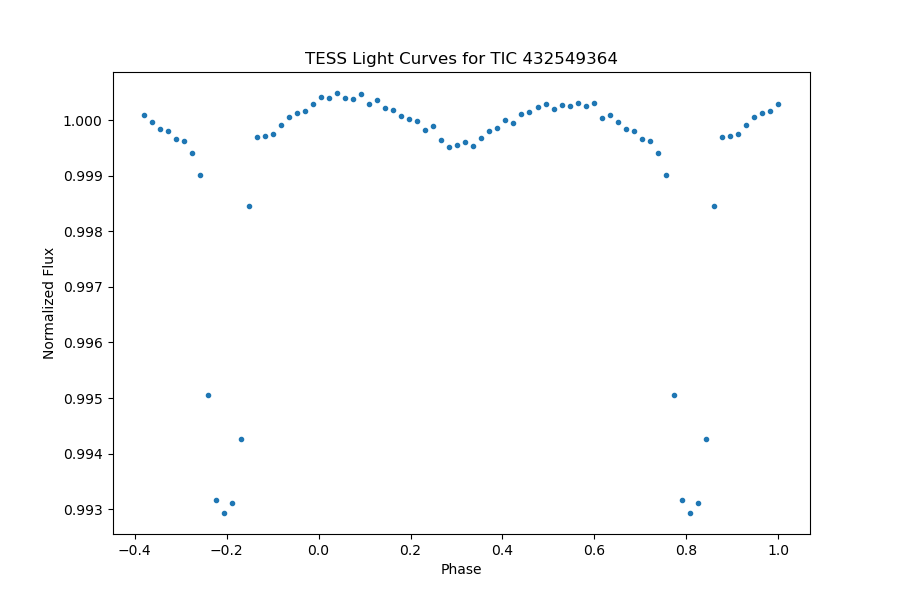
\includegraphics[width=0.7\linewidth]{image/432549364_folded.png}\captionsetup{font=small} \caption{The full phase-folded light curve of TIC 432549364, planetary transit is very clear and the secondary eclipse can be identified significantly.}\label{fig:432549364_folded}\end{figure}\begin{figure}[H]\centering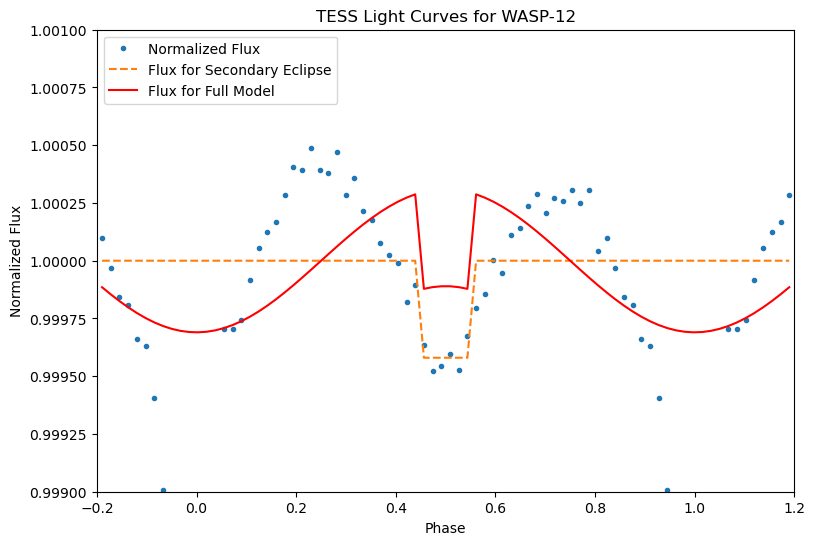
\includegraphics[width=0.65\linewidth]{image/432549364.png}\captionsetup{font=small} \caption{A close review of the phase-folded light curve of TIC 432549364, the models of secondary eclipse and day-night modulation are presented.}\label{fig:432549364}\end{figure}
\newpage
The planet TIC 236445129 has an orbital period of 0.9689943 days, showing significant transit with a depth of 0.01456\% and a transit duration of 2.295 hours. The secondary eclipse can be identified significantly in the full phase-folded light curve Figure \ref{fig:236445129_folded}. A close review of the light curve outside of transit Figure \ref{fig:236445129}, we fit the light curve with models of the secondary eclipse and day-night modulation.\begin{figure}[H]\centering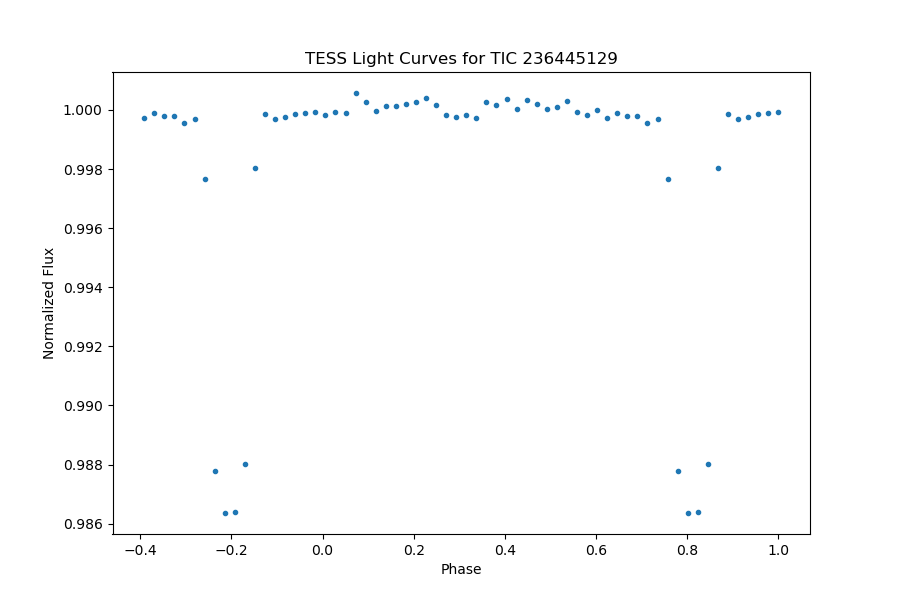
\includegraphics[width=0.7\linewidth]{image/236445129_folded.png}\captionsetup{font=small} \caption{The full phase-folded light curve of TIC 236445129, planetary transit is very clear and the secondary eclipse can be identified significantly.}\label{fig:236445129_folded}\end{figure}\begin{figure}[H]\centering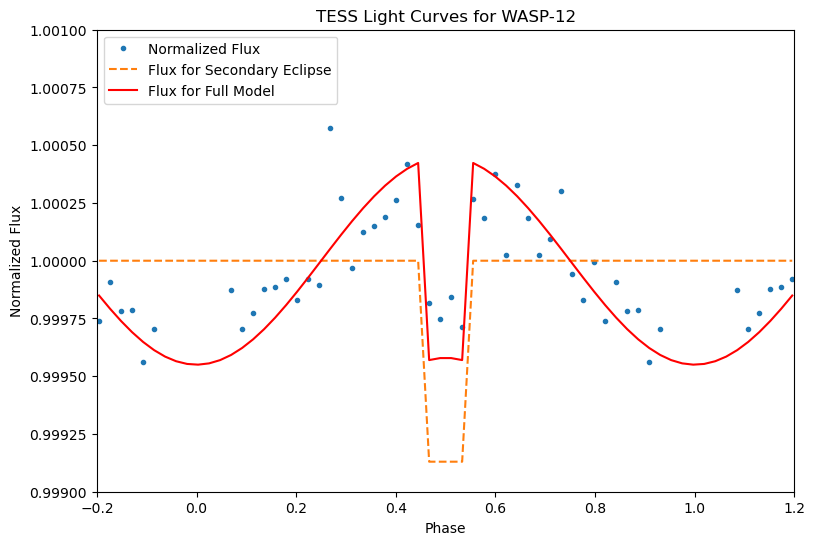
\includegraphics[width=0.65\linewidth]{image/236445129.png}\captionsetup{font=small} \caption{A close review of the phase-folded light curve of TIC 236445129, the models of the secondary eclipse and day-night modulation are presented.}\label{fig:236445129}\end{figure}
\newpage
The planet TIC 158324245 has an orbital period of 1.763588814 days, showing significant transit with a depth of 0.008089230752\% and a transit duration of 3.251584895 hours. The secondary eclipse can be identified significantly in the full phase-folded light curve Figure \ref{fig:158324245_folded}. A close review of the light curve outside of transit Figure \ref{fig:158324245}, we fit the light curve with models of secondary eclipse and day-night modulation\begin{figure}[H]\centering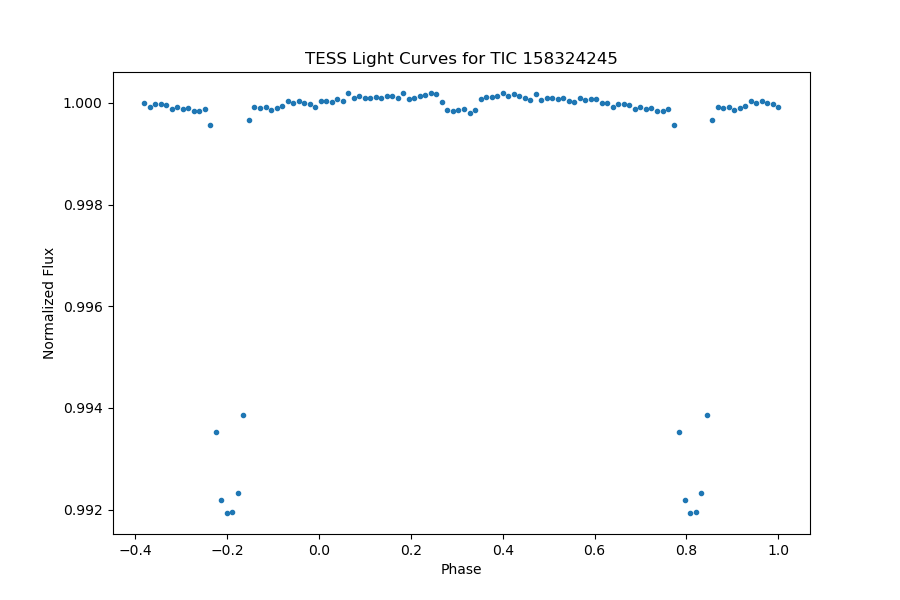
\includegraphics[width=0.7\linewidth]{image/158324245_folded.png}\captionsetup{font=small} \caption{The full phase-folded light curve of TIC 158324245, planetary transit is very clear and the secondary eclipse can be identified significantly.}\label{fig:158324245_folded}\end{figure}\begin{figure}[H]\centering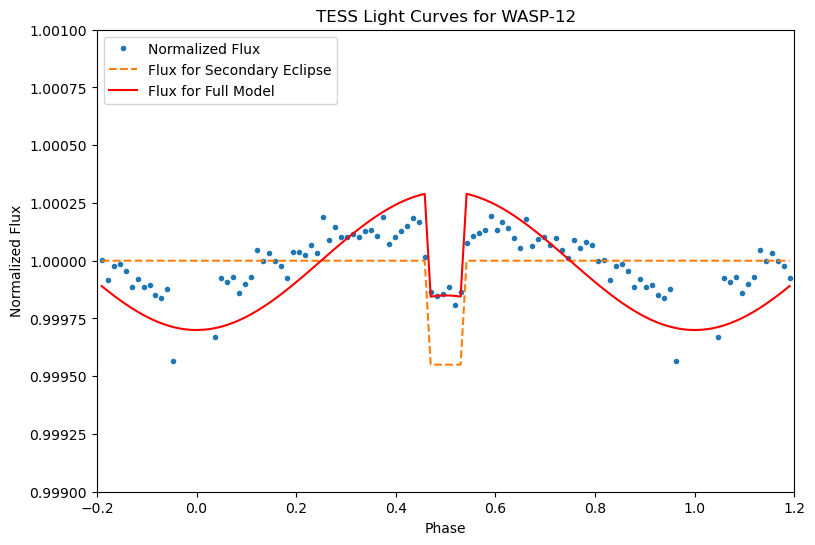
\includegraphics[width=0.65\linewidth]{image/158324245.png}\captionsetup{font=small} \caption{A close review of the phase-folded light curve of TIC 158324245, the models of secondary eclipse and day-night modulation are presented.}\label{fig:158324245}\end{figure}
\newpage
The planet TIC 293435336 has an orbital period of 1.809881077 days, showing significant transit with a depth of 0.01303356127\% and a transit duration of 3.763662407 hours. The secondary eclipse can be identified significantly in the full phase-folded light curve Figure \ref{fig:293435336_folded}. A close review of the light curve outside of transit Figure \ref{fig:293435336}, we fit the light curve with models of secondary eclipse and day-night modulation.\begin{figure}[H]\centering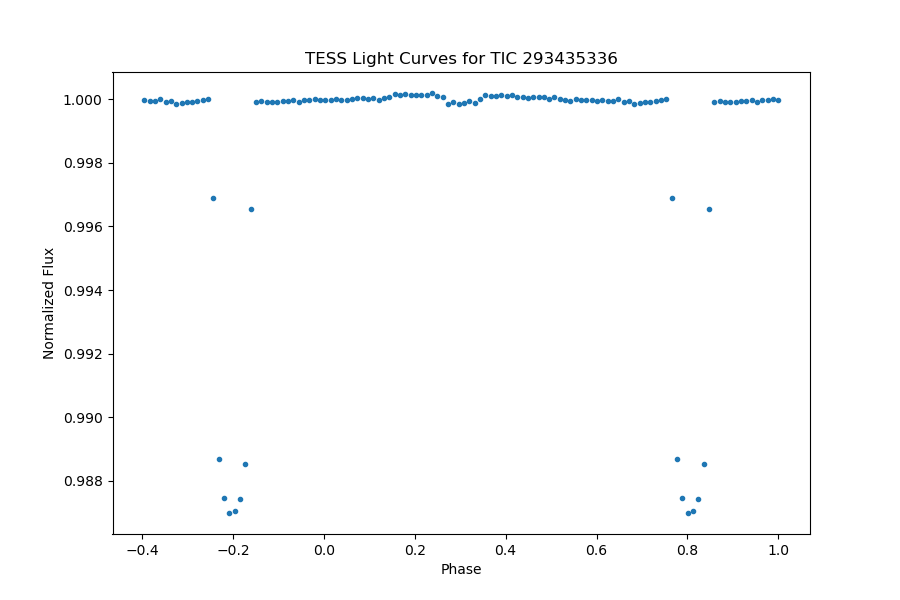
\includegraphics[width=0.7\linewidth]{image/293435336_folded.png}\captionsetup{font=small} \caption{The full phase-folded light curve of TIC 293435336, planetary transit is very clear and the secondary eclipse can be identified significantly.}\label{fig:293435336_folded}\end{figure}\begin{figure}[H]\centering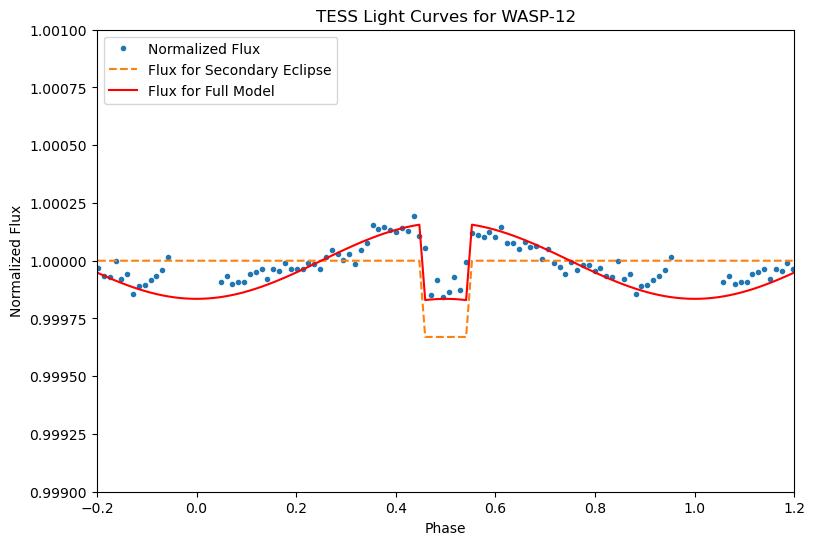
\includegraphics[width=0.65\linewidth]{image/293435336.png}\captionsetup{font=small} \caption{A close review of the phase-folded light curve of TIC 293435336, the models of secondary eclipse and day-night modulation are presented.}\label{fig:293435336}\end{figure}
\newpage
The planet TIC 424865156 has an orbital period of 2.2047975 days, showing significant transit with a depth of 0.00658\% and a transit duration of 3.956 hours. The secondary eclipse can be identified significantly in the full phase-folded light curve Figure \ref{fig:424865156_folded}. A close review of the light curve outside of transit Figure \ref{fig:424865156}, we fit the light curve with models of the secondary eclipse and day-night modulation.\begin{figure}[H]\centering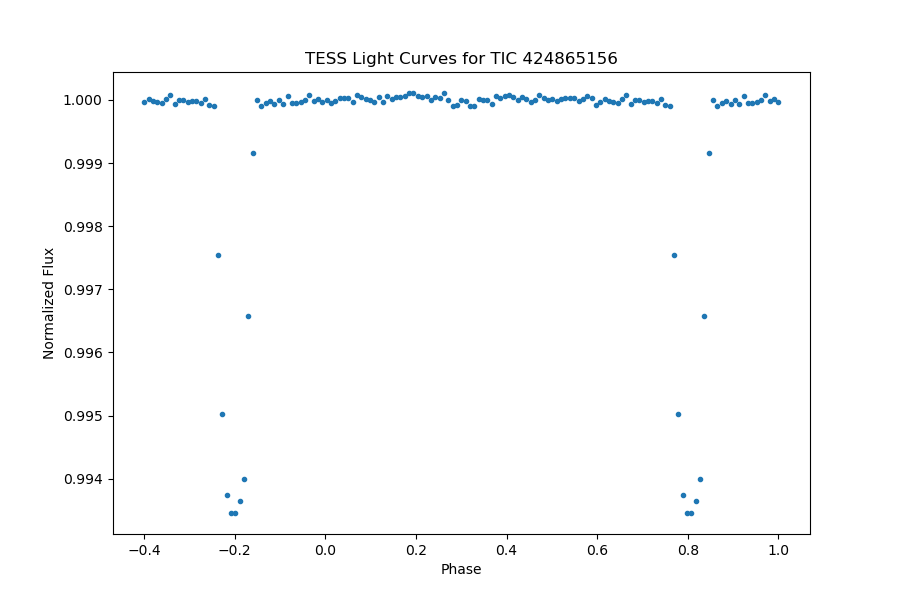
\includegraphics[width=0.7\linewidth]{image/424865156_folded.png}\captionsetup{font=small} \caption{The full phase-folded light curve of TIC 424865156, planetary transit is very clear and the secondary eclipse can be identified significantly.}\label{fig:424865156_folded}\end{figure}\begin{figure}[H]\centering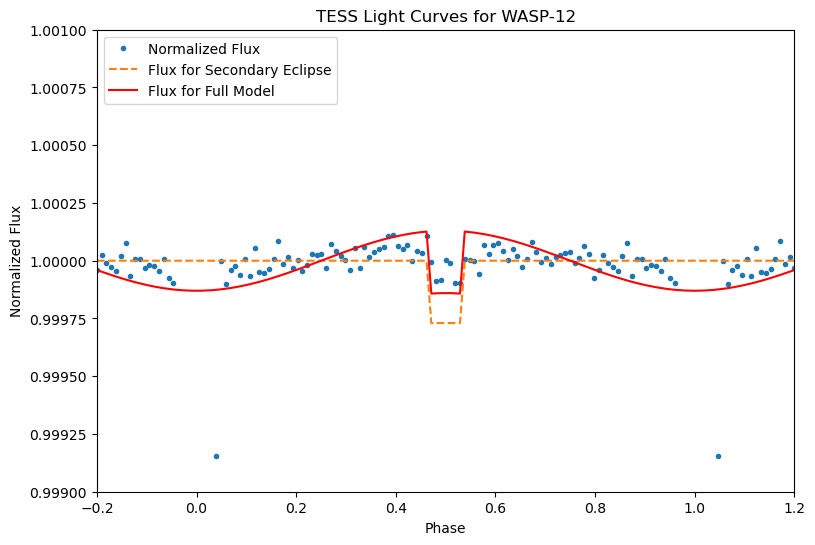
\includegraphics[width=0.65\linewidth]{image/424865156.png}\captionsetup{font=small} \caption{A close review of the phase-folded light curve of TIC 424865156, the models of the secondary eclipse and day-night modulation are presented.}\label{fig:424865156}\end{figure}
\newpage
The planet TIC 100100827 has an orbital period of 0.941451622 days, showing significant transit with a depth of 0.01062754164\% and a transit duration of 2.157561137 hours. The secondary eclipse can be identified significantly in the full phase-folded light curve Figure \ref{fig:100100827_folded}. A close review of the light curve outside of transit Figure \ref{fig:100100827}, we fit the light curve with models of the secondary eclipse and day-night modulation.\begin{figure}[H]\centering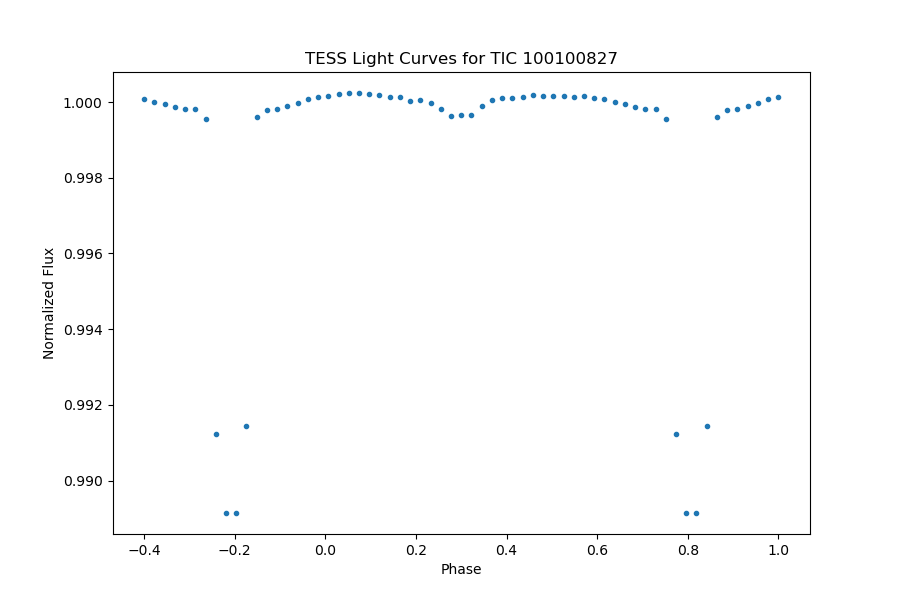
\includegraphics[width=0.7\linewidth]{image/100100827_folded.png}\captionsetup{font=small} \caption{The full phase-folded light curve of TIC 100100827, planetary transit is very clear and the secondary eclipse can be identified significantly.}\label{fig:100100827_folded}\end{figure}\begin{figure}[H]\centering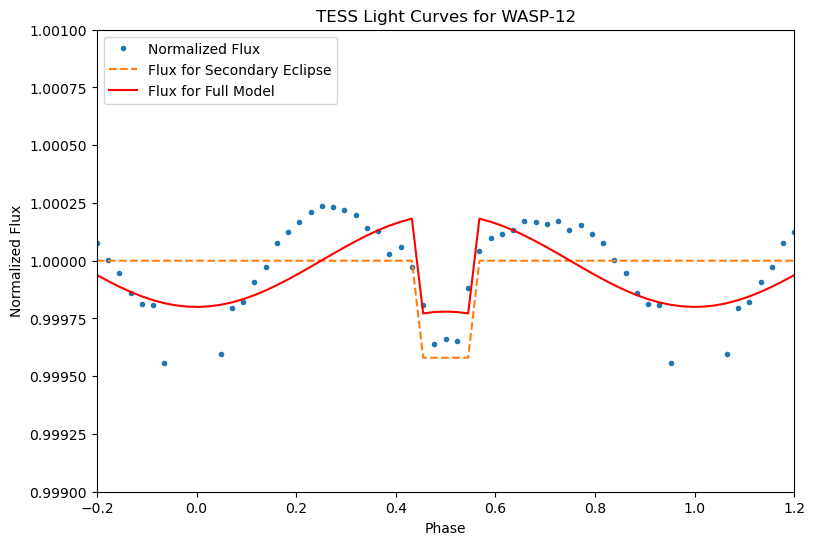
\includegraphics[width=0.65\linewidth]{image/100100827.png}\captionsetup{font=small} \caption{A close review of the phase-folded light curve of TIC 100100827, the models of the secondary eclipse and day-night modulation are presented.}\label{fig:100100827}\end{figure}
\newpage
\subsubsection{Objects that are different from our expectations and model}

The planet TIC 129979528 has an orbital period of 1.219867856 days, showing significant transit with a depth of 0.01347480502\% and a transit duration of 2.860252706 hours. The secondary eclipse can be identified significantly in the full phase-folded light curve Figure \ref{fig:129979528_folded}. A close review of the light curve outside of transit Figure \ref{fig:129979528}, we fit the light curve with models of the secondary eclipse and day-night modulation.\begin{figure}[H]\centering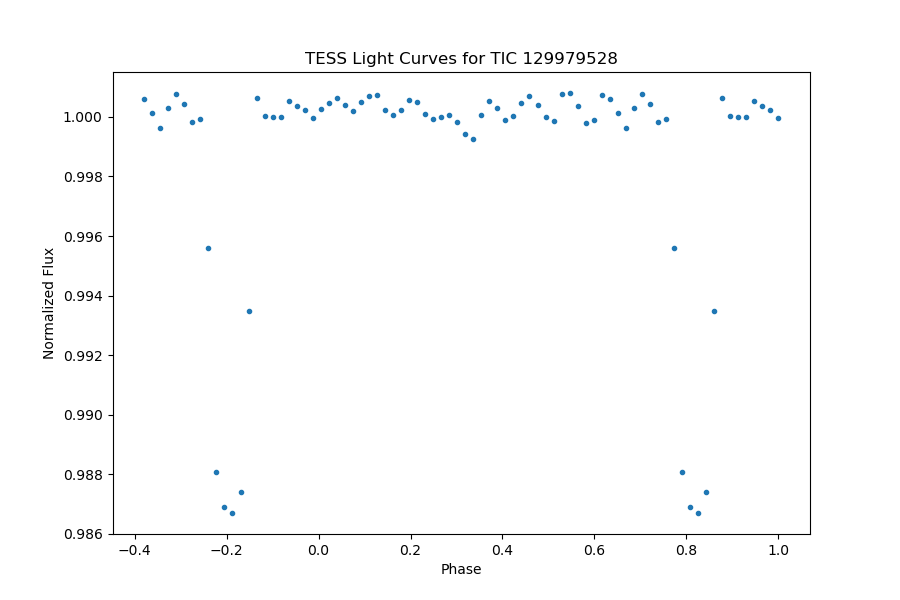
\includegraphics[width=0.7\linewidth]{image/129979528_folded.png}\captionsetup{font=small} \caption{The full phase-folded light curve of TIC 129979528, planetary transit is very clear and the secondary eclipse can be identified significantly.}\label{fig:129979528_folded}\end{figure}\begin{figure}[H]\centering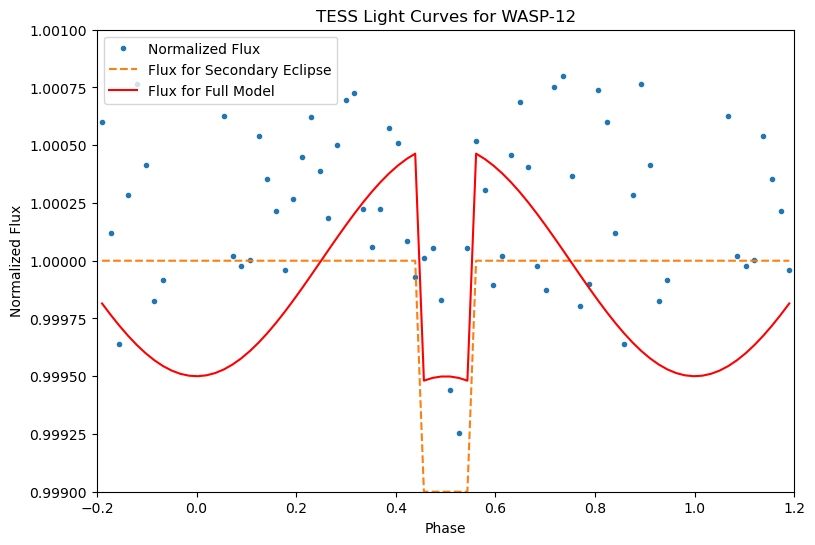
\includegraphics[width=0.65\linewidth]{image/129979528.png}\captionsetup{font=small} \caption{A close review of the phase-folded light curve of TIC 129979528, the models of the secondary eclipse and day-night modulation are presented.}\label{fig:129979528}\end{figure}
\newpage
The planet TIC 293687315 has an orbital period of 2.8716968 days, showing significant transit with a depth of 0.00868\% and a transit duration of 4.541 hours. The secondary eclipse can be identified significantly in the full phase-folded light curve Figure \ref{fig:293687315_folded}. A close review of the light curve outside of transit Figure \ref{fig:293687315}, we fit the light curve with models of the secondary eclipse and day-night modulation.\begin{figure}[H]\centering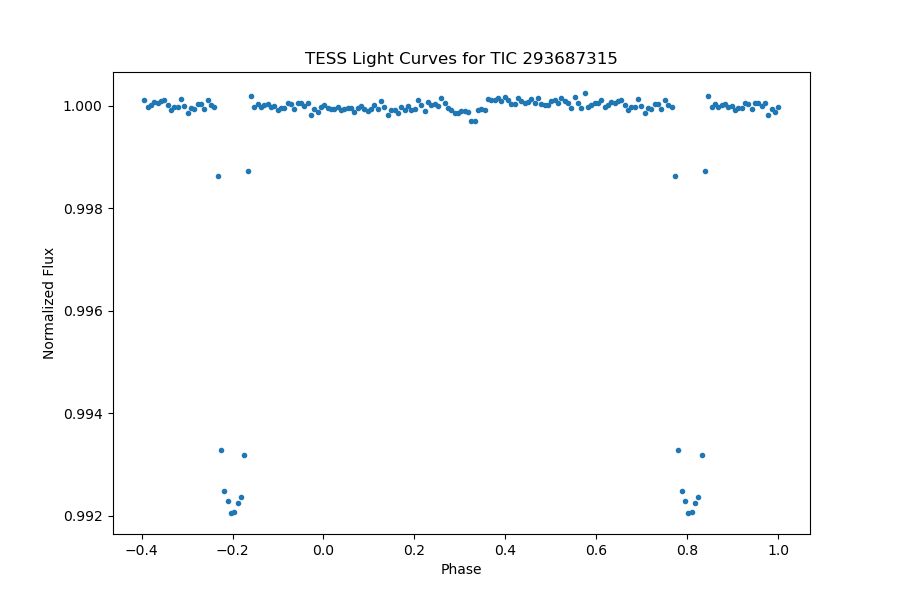
\includegraphics[width=0.7\linewidth]{image/293687315_folded.png}\captionsetup{font=small} \caption{The full phase-folded light curve of TIC 293687315, planetary transit is very clear and the secondary eclipse can be identified significantly.}\label{fig:293687315_folded}\end{figure}\begin{figure}[H]\centering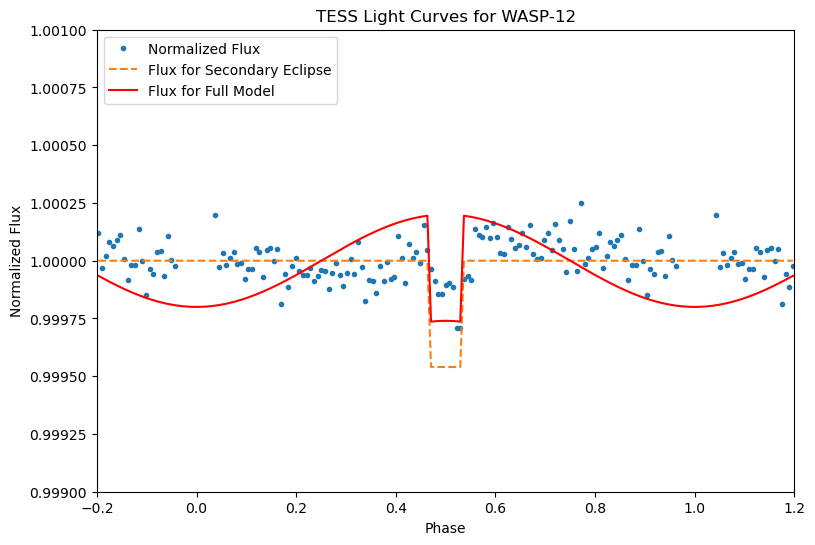
\includegraphics[width=0.65\linewidth]{image/293687315.png}\captionsetup{font=small} \caption{A close review of the phase-folded light curve of TIC 293687315, the models of secondary eclipse and day-night modulation are presented.}\label{fig:293687315}\end{figure}
\newpage
The planet TIC 35516889 has an orbital period of 0.788839248 days, showing significant transit with a depth of 0.02243191516\% and a transit duration of 1.596710714 hours. The secondary eclipse can be identified significantly in the full phase-folded light curve Figure \ref{fig:35516889_folded}. A close review of the light curve outside of transit Figure \ref{fig:35516889}, we fit the light curve with models of the secondary eclipse and day-night modulation.\begin{figure}[H]\centering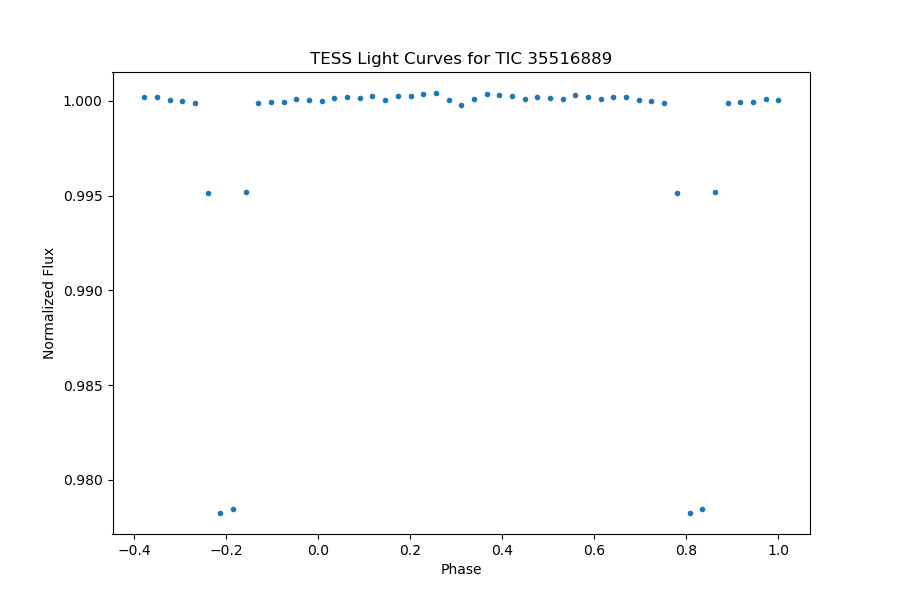
\includegraphics[width=0.7\linewidth]{image/35516889_folded.png}\captionsetup{font=small} \caption{The full phase-folded light curve of TIC 35516889, planetary transit is very clear and the secondary eclipse can be identified significantly.}\label{fig:35516889_folded}\end{figure}\begin{figure}[H]\centering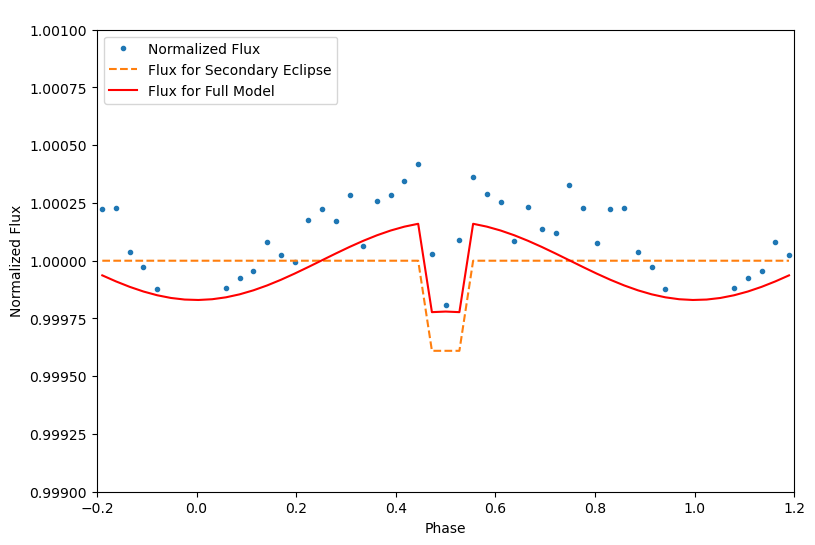
\includegraphics[width=0.65\linewidth]{image/35516889.png}\captionsetup{font=small} \caption{A close review of the phase-folded light curve of TIC 35516889, the models of the secondary eclipse and day-night modulation are presented.}\label{fig:35516889}\end{figure}
\newpage
The planet TIC 371443216 has an orbital period of 2.8240691 days, showing significant transit with a depth of 0.00897\% and a transit duration of 3.808 hours. The secondary eclipse can be identified significantly in the full phase-folded light curve Figure \ref{fig:371443216_folded}. A close review of the light curve outside of transit Figure \ref{fig:371443216}, we fit the light curve with models of the secondary eclipse and day-night modulation.\begin{figure}[H]\centering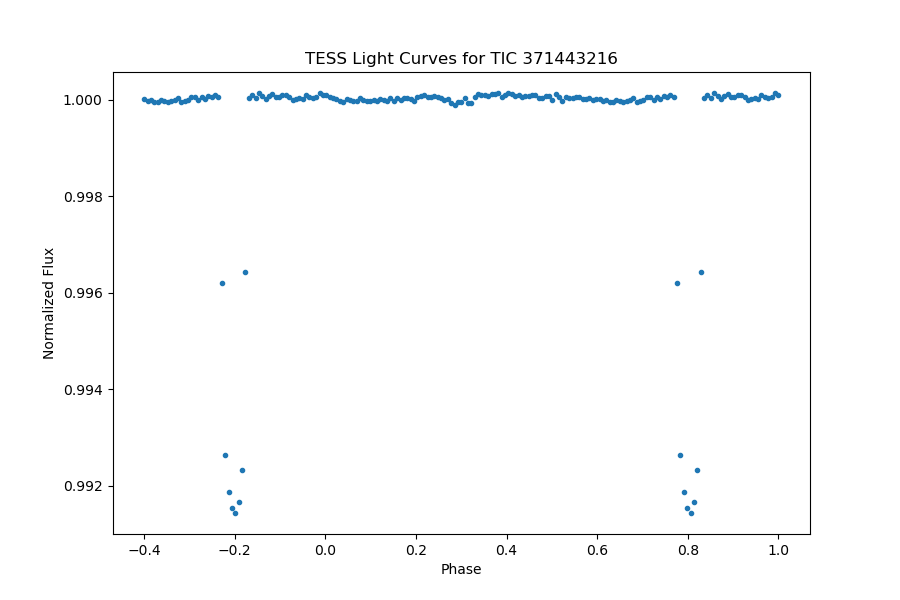
\includegraphics[width=0.7\linewidth]{image/371443216_folded.png}\captionsetup{font=small} \caption{The full phase-folded light curve of TIC 371443216, planetary transit is very clear and the secondary eclipse can be identified significantly.}\label{fig:371443216_folded}\end{figure}\begin{figure}[H]\centering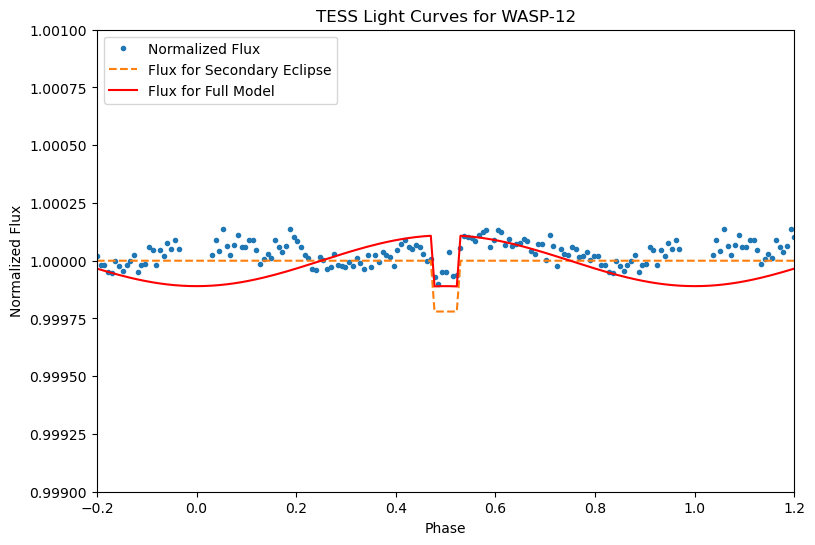
\includegraphics[width=0.65\linewidth]{image/371443216.png}\captionsetup{font=small} \caption{A close review of the phase-folded light curve of TIC 371443216, the models of the secondary eclipse and day-night modulation are presented.}\label{fig:371443216}\end{figure}
\newpage
\section{Conclusion}

    In this comprehensive study, we have undertaken the development of an exceptionally efficient and advanced Python program that aims to revolutionize the analysis of TESS (Transiting Exoplanet Survey Satellite) light curves. Our program is specifically designed to search for and identify the secondary eclipse and day-night modulation phenomena in a vast dataset comprising over 400 known short-period transiting exoplanets.

    One of the key highlights of our program is its remarkable capability to automatically detect and discard low-quality photometric data points within the light curves. By implementing this feature, we ensure that our analysis is based on robust and reliable data, thereby enhancing the accuracy and validity of our findings.

    Following the removal of unreliable data points, the remaining high-quality light curves are meticulously folded into orbital phases, precisely determined by the primary transits. This innovative phase-folding technique enables us to generate exquisitely detailed and precise phase-folded average light curves, which are exceptionally well-suited for detecting and studying the secondary eclipse and day-night modulation phenomena.

    Through the implementation of our cutting-edge program, we have achieved unprecedented success in identifying and characterizing planetary reflection in an astounding 17 transiting exoplanetary systems. This impressive sample size significantly surpasses the current number of identified exoplanets by a factor of two, underscoring the substantial impact and novelty of our research.

    Moreover, our rigorous analysis has not been confined solely to the identification of planetary reflection. We have also successfully detected and analyzed other crucial orbital-phase variations within the light curves of our extensive sample. These variations include modulations arising from the ellipsoidal effect and relativistic beaming effect, providing invaluable insights into the physical properties, atmospheric composition, accurate mass, and orbital evolution of these remarkable exoplanetary systems.

    Looking ahead, we have ambitious plans to further refine and upgrade our pioneering Python program. Our ultimate goal is to extend its functionality and capabilities to encompass the search for and analysis of orbital-phase modulations in non-transiting exoplanets. Leveraging the exceptional precision and accuracy of TESS photometry, we anticipate making more discoveries, including the identification of previously unknown exoplanets and the precise determination of accurate masses for known exoplanets.

\section{Extra material}

\begin{figure}[H]
    \centering
    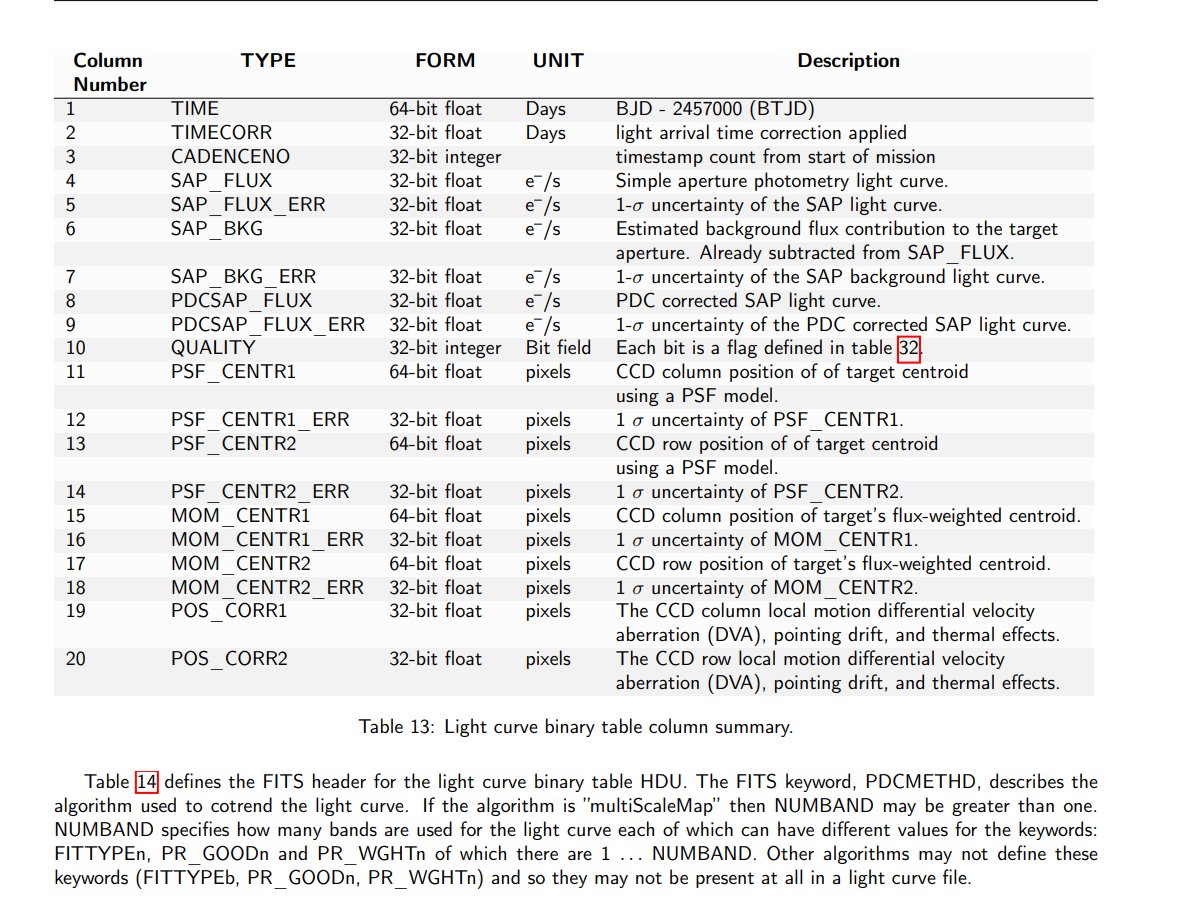
\includegraphics[width=0.8\linewidth]{image/EXM_Table13.jpg}
    \label{fig:table13}
\end{figure}

\newpage
\addcontentsline{toc}{section}{References}
\begin{thebibliography}{}

\bibitem[Guerrero et al.(2021)]{guerrero2021} Guerrero, N. M., et al. 2021, ApJS, 254, 39

\bibitem[Mayor \& Queloz(1995)]{mayor1995} Mayor, M., \& Queloz, D. 1995, Nature, 378, 6555

\bibitem[Perryman(2018)]{perryman2018} Perryman, M. 2018, \textit{The Exoplanet Handbook by Michael Perryman}, Cambridge University Press, Second Edition

\bibitem[The Royal Swedish Academy of Sciences(2019)]{nobel2019} The Royal Swedish Academy of Sciences. 2019, \textit{Scientific Background on the Nobel Prize in Physics 2019}

\bibitem[Twichen et al.(2020)]{twichen2020} Twichen, J. D., et al. 2020, \textit{TESS Science Data Products Description Document}

\bibitem[Vanderspeck et al.(2018)]{vanderspeck2018} Vanderspeck, R., et al. 2018, \textit{TESS Instrument Handbook}


\bibitem[Wong et al.(2019)]{wong2019} Wong, I., et al. 2019, The Astronomical Journal, 159, 104


\bibitem[Wong et al.(2020)]{wong2020} Wong, I., et al. 2020, The Astronomical Journal, 160, 155

\bibitem[Wong et al.(2021)]{wong2021} Wong, I., et al. 2021, The Astronomical Journal, 162, 127

\bibitem[Yee et al.(2020)]{yee2020} Yee, S. W., Winn, J. N., Knutson, H. A., et al. 2020, ApJL, 888, L5

\end{thebibliography}

\newpage
\addcontentsline{toc}{section}{Acknowledgement}
\section*{Acknowledgement}
We would like to express our sincere gratitude to Mrs Yang Ningyu for her patient guidance and advice throughout this research project. His insightful suggestions and domain expertise were invaluable in enabling us to carry out the analysis of exoplanet phase curves.
We also wish to acknowledge the computing facilities provided by the secondary school computer lab, without which this intensive data processing work would not have been feasible. The availability of sufficient computational resources was crucial to the successful derivation of the results presented here.
The support we received throughout the research and analysis process was important in overcoming challenges and keeping the project on track. We truly appreciate the time and effort dedicated by Mrs Yang and the computing lab staff.

\end{document}